%%% LaTeX-Vorlage Version 1.8 %%%

% Grundlegende Dokumenteneigenschaften gemäß DHBW-Vorgaben
\documentclass[a4paper,fontsize=11pt,oneside,parskip=half,headings=normal]{scrreprt} 
% \usepackage{showframe} % nur für Kontrolle der Ränder 

%%% Präambel einbinden (mit Festlegungen gemäß DHBW-Vorgaben) %%%
%%% Präambel %%%
% hier sollten keine Änderungen erforderlich sein
%
\usepackage[utf8]{inputenc}   % Zeichencodierung UTF-8 für Eingabe-Dateien
\usepackage[T1]{fontenc}      % Darstellung von Umlauten im PDF

\usepackage{listings}         % für Einbindung von Code-Listings
\lstset{numbers=left,numberstyle=\tiny,numbersep=5pt,texcl=true}
\lstset{literate=             % erlaubt Sonderzeichen in Code-Listings 
{Ö}{{\"O}}1
{Ä}{{\"A}}1
{Ü}{{\"U}}1
{ß}{{\ss}}2
{ü}{{\"u}}1
{ä}{{\"a}}1
{ö}{{\"o}}1
{€}{{\euro}}1
}

\usepackage[
  inner=35mm,outer=15mm,top=25mm,
  bottom=20mm,foot=12mm,includefoot
]{geometry}                 % Einstellungen für Ränder

\usepackage{float}

\usepackage[ngerman]{babel} % Spracheinstellungen Deutsch
\usepackage{minted}
\usepackage[babel,german=quotes]{csquotes} % deutsche Anf.zeichen
\usepackage{enumerate}      % anpassbare Nummerier./Aufz.
\usepackage{graphicx}       % Einbinden von Grafiken
\usepackage[onehalfspacing]{setspace} % anderthalbzeilig
\usepackage{color}          % Verwendung von Farbe 

\usepackage{acronym}        % für ein Abkürzungsverzeichnis

\usepackage{lscape}

\usepackage[                % Biblatex
  backend=biber,
  bibstyle=_dhbw_authoryear,maxbibnames=99,
  citestyle=authoryear,     
  uniquename=true, useprefix=true, dashed=false,
  bibencoding=utf8, giveninits=true]{biblatex}
%kein Punkt am Ende bei \footcite
%http://www.golatex.de/footcite-ohne-punkt-am-schluss-t4865.html
\renewcommand{\bibfootnotewrapper}[1]{\bibsentence#1}


%Reihenfolge der Autorennamen
%   
% http://golatex.de/viewtopic,p,80448.html#80448
% Argumente: siehe http://texwelt.de/blog/modifizieren-eines-biblatex-stils/
\DeclareNameFormat{sortname}{% Bibliographie
  \ifnum\value{uniquename}=0 % Normalfall
    \ifuseprefix%
      {%
         \usebibmacro{name:family-given}
           {\namepartfamily}
           {\namepartgiveni}
           {\namepartprefix}
           {\namepartsuffixi}%
       }
      {%
         \usebibmacro{name:family-given}
           {\namepartfamily}
           {\namepartgiveni}
           {\namepartprefixi}
           {\namepartsuffixi}%
       }%
  \fi
  \ifnum\value{uniquename}=1% falls nicht eindeutig, abgek. Vorname 
      {%
         \usebibmacro{name:family-given}
           {\namepartfamily}
           {\namepartgiveni}
           {\namepartprefix}
           {\namepartsuffix}%
       }%
  \fi
  \ifnum\value{uniquename}=2% falls nicht eindeutig, ganzer Vorname 
      {%
         \usebibmacro{name:family-given}
           {\namepartfamily}
           {\namepartgiven}
           {\namepartprefix}
           {\namepartsuffix}%
       }%
  \fi   
  \usebibmacro{name:andothers}}

\DeclareNameFormat{labelname}{% für Zitate
  \ifnum\value{uniquename}=0 % Normalfall
    \ifuseprefix%
      {%
         \usebibmacro{name:family-given}
           {\namepartfamily}
           {\empty}
           {\namepartprefix}
           {\namepartsuffixi}%
       }
      {%
         \usebibmacro{name:family-given}
           {\namepartfamily}
           {\empty}
           {\namepartprefixi}
           {\namepartsuffixi}%
       }%
  \fi
  \ifnum\value{uniquename}=1% falls nicht eindeutig, abgek. Vorname 
      {%
         \usebibmacro{name:family-given}
           {\namepartfamily}
           {\namepartgiveni}
           {\namepartprefix}
           {\namepartsuffix}%
       }%
  \fi
  \ifnum\value{uniquename}=2% falls nicht eindeutig, ganzer Vorname 
      {%
         \usebibmacro{name:family-given}
           {\namepartfamily}
           {\namepartgiven}
           {\namepartprefix}
           {\namepartsuffix}%
       }%
  \fi   
  \usebibmacro{name:andothers}}
      
  
\DeclareFieldFormat{extrayear}{% = the 'a' in 'Jones 1995a'
  \iffieldnums{labelyear}
    {\mknumalph{#1}}
    {\mknumalph{#1}}}        

\renewcommand*{\multinamedelim}{\addslash}
\renewcommand*{\finalnamedelim}{\addslash}
\renewcommand*{\multilistdelim}{\addslash}
\renewcommand*{\finallistdelim}{\addslash}

\renewcommand{\nameyeardelim}{~}

% Literaturverzeichnis: Doppelpunkt zwischen Name (Jahr): Rest 
% http://de.comp.text.tex.narkive.com/Tn1HUIXB/biblatex-authoryear-und-doppelpunkt
\renewcommand{\labelnamepunct}{\addcolon\addspace}

% damit die Darstellung für Vollzitate von Primärquellen in 
% Fußnoten später auf "nicht fett" geändert werden kann 
% (nur für Zitate von Sekundärliteratur relevant)
\newcommand{\textfett}[1]{\textbf{#1}}

% für Zitate von Sekundärliteratur:
\newcommand{\footcitePrimaerSekundaer}[4]{%
  \renewcommand{\textfett}[1]{##1}%
  \footnote{\fullcite[#2]{#1}, zitiert nach \cite[#4]{#3}}%  
  \renewcommand{\textfett}[1]{\textbf{##1}}%
}

% Im Literaturverzeichnis: Autor (Jahr) fett
\renewbibmacro*{author}{%
  \ifboolexpr{%
    test \ifuseauthor%
    and
    not test {\ifnameundef{author}}
  }
    {\usebibmacro{bbx:dashcheck}
       {\bibnamedash}
       {\usebibmacro{bbx:savehash}%
        \textfett{\printnames{author}}%
        \iffieldundef{authortype}
          {\setunit{\addspace}}
          {\setunit{\addcomma\space}}}%
     \iffieldundef{authortype}
       {}
       {\usebibmacro{authorstrg}%
        \setunit{\addspace}}}%
    {\global\undef\bbx@lasthash
     \usebibmacro{labeltitle}%
     \setunit*{\addspace}}%
  \textfett{\usebibmacro{date+extrayear}}}

% Sonderfall: Quelle ohne Autor, aber mit Herausgeber
% Name des Herausgebers wird fett gedruckt
\renewbibmacro*{bbx:editor}[1]{%
  \ifboolexpr{%
    test \ifuseeditor%
    and
    not test {\ifnameundef{editor}}
  }
    {\usebibmacro{bbx:dashcheck}
       {\bibnamedash}
       {\textfett{\printnames{editor}}%
        \setunit{\addcomma\space}%
        \usebibmacro{bbx:savehash}}%
     \usebibmacro{#1}%
     \clearname{editor}%
     \setunit{\addspace}}%
    {\global\undef\bbx@lasthash
     \usebibmacro{labeltitle}%
     \setunit*{\addspace}}%
  \textfett{\usebibmacro{date+extrayear}}}

% Anpassungen für deutsche Sprache
\DefineBibliographyStrings{ngerman}{% 
	nodate = {{o.J.}},
	urlseen = {{Abruf:}},
	ibidem = {{ebenda}}
}

% keine Anführungszeichen beim Titel im Literaturverzeichnis
\DeclareFieldFormat[article,book,inbook,incollection,inproceedings,manual,misc,phdthesis,thesis,online,report]{title}{#1\isdot}

\newcommand{\literaturverzeichnis}{%
% nur Literaturverzeichnis
% (als eigenes Kapitel)
\phantomsection
\addcontentsline{toc}{chapter}{Literaturverzeichnis}
\spezialkopfzeile{Literaturverzeichnis}
\defbibheading{lit}{\chapter*{Literaturverzeichnis}}
\label{chapter:quellen}
\printbibliography[heading=lit,notkeyword=ausblenden]
} % mit DHBW-spezifischen Einstellungen



\usepackage{hyperref}       % URL-Formatierung, klickbare Verweise

% \usepackage[plain]{algorithm}
% \usepackage{algorithmic}

\usepackage{tocloft}        % für Verzeichnis der Anhänge

\newcounter{anhcnt}
\setcounter{anhcnt}{0}
\newlistof{anhang}{app}{}

\newcommand{\anhang}[1]{%
  \refstepcounter{anhcnt}
  \setcounter{anhteilcnt}{0}
  \section*{Anhang \theanhcnt: #1}
  \addcontentsline{app}{section}{\protect\numberline{Anhang \theanhcnt}#1}\par
}

\newcounter{anhteilcnt}
\setcounter{anhteilcnt}{0}

\newcommand{\anhangteil}[1]{%
	\refstepcounter{anhteilcnt}
	\subsection*{Anhang~\arabic{anhcnt}/\arabic{anhteilcnt}: #1}
	\addcontentsline{app}{subsection}{\protect\numberline{Anhang \theanhcnt/\arabic{anhteilcnt}}#1}\par
}

\renewcommand{\theanhteilcnt}{Anhang \theanhcnt/\arabic{anhteilcnt}}

% vgl. S. 4 Paket-Beschreibung tocloft 	
% Einrückungen für Anhangverzeichnis
\makeatletter
\newcommand{\abstaendeanhangverzeichnis}{
\renewcommand*{\l@section}{\@dottedtocline{1}{0em}{5.5em}}
\renewcommand*{\l@subsection}{\@dottedtocline{2}{2.3em}{6.5em}}
}
\makeatother

% Abbildungs- und Tabellenverzeichnis
% Bezeichnungen
\renewcaptionname{ngerman}{\figurename}{Abb.}
\renewcaptionname{ngerman}{\tablename}{Tab.}
% Einrückungen
\makeatletter
\renewcommand*{\l@figure}{\@dottedtocline{1}{0em}{2.3em}}
\renewcommand*{\l@table}{\@dottedtocline{1}{0em}{2.3em}}
\makeatother



\usepackage{tabularx}

\usepackage{chngcntr}                % fortlaufende Zähler für Fußnoten, Abbildungen und Tabellen
\counterwithout{figure}{chapter}
\counterwithout{table}{chapter}
\counterwithout{footnote}{chapter}

\usepackage[automark]{scrlayer-scrpage} 
%% Definitionen für Kopf- und Fußzeile auf normalen Seiten
\defpagestyle{kopfzeile}
{% Kopfdefinition
  (\textwidth,0pt)    % Länge der oberen Linie,Dicke der oberen Linie       
  {} % Definition für linke Seiten im doppelseitigen Layout
  {} % Definition für rechte Seiten im doppelseitigen Layout      
  {  % Definition für Seiten im einseitigen Layout
	\makebox[0pt][l]{\rightmark}% 
	\makebox[\linewidth]{}% 
  }        
  (\textwidth, 0.4pt) % Untere Linienlänge, Untere Liniendicke
}
{% Fußdefinition
  (\textwidth,0pt)    % Obere Linienlänge, Obere Liniendicke
  {} % Definition für linke Seiten im doppelseitigen Layout
  {} % Definition für rechte Seiten im doppelseitigen Layout
  {  % Definition für Seiten im einseitigen Layout
    \makebox[\linewidth]{}%
    \makebox[0pt][r]{\pagemark}%
  }
  (\textwidth, 0pt)   % Länge der unteren Linie,Dicke der unteren Linie
}

%% Definitionen für Kopf- und Fußzeile auf ersten Seiten eines Kapitels
\defpagestyle{kapitelkopfzeile}
{% Kopfdefinition
  (\textwidth,0pt)    % Länge der oberen Linie,Dicke der oberen Linie       
  {} % Definition für linke Seiten im doppelseitigen Layout
  {} % Definition für rechte Seiten im doppelseitigen Layout      
  {}  % Definition für Seiten im einseitigen Layout
  (\textwidth, 0pt) % Untere Linienlänge, Untere Liniendicke
}
{% Fußdefinition
  (\textwidth,0pt)    % Obere Linienlänge, Obere Liniendicke
  {} % Definition für linke Seiten im doppelseitigen Layout
  {} % Definition für rechte Seiten im doppelseitigen Layout
  {  % Definition für Seiten im einseitigen Layout
    \makebox[\linewidth]{}%
    \makebox[0pt][r]{\pagemark}%
  }
  (\textwidth, 0pt)   % Länge der unteren Linie,Dicke der unteren Linie
}

%% Definitionen für Kopf- und Fußzeile im Anhang und bei Quellenverzeichnisse
\newcommand{\spezialkopfzeileBezeichnung}{}
\defpagestyle{spezialkopfzeile}
{% Kopfdefinition
  (\textwidth,0pt)    % Länge der oberen Linie,Dicke der oberen Linie       
  {} % Definition für linke Seiten im doppelseitigen Layout
  {} % Definition für rechte Seiten im doppelseitigen Layout      
  {  % Definition für Seiten im einseitigen Layout
	\makebox[0pt][l]{\spezialkopfzeileBezeichnung}% 
	\makebox[\linewidth]{}% 
  }        
  (\textwidth, 0.4pt) % Untere Linienlänge, Untere Liniendicke
}
{% Fußdefinition
  (\textwidth,0pt)    % Obere Linienlänge, Obere Liniendicke
  {} % Definition für linke Seiten im doppelseitigen Layout
  {} % Definition für rechte Seiten im doppelseitigen Layout
  {  % Definition für Seiten im einseitigen Layout
    \makebox[\linewidth]{}%
    \makebox[0pt][r]{\pagemark}%
  }
  (\textwidth, 0pt)   % Länge der unteren Linie,Dicke der unteren Linie
}
            
\newcommand\spezialkopfzeile[1]{%
  \renewcommand\spezialkopfzeileBezeichnung{#1}
  \pagestyle{spezialkopfzeile}
}
                
% Standard-Pagestyle auswählen
\pagestyle{kopfzeile}

% keine Kopfzeile anzeigen auf Seiten, auf denen ein 
% Kapitel beginnt oder das Inhalts-/Abbildungs-/Tabellenverzeichnis steht 
\renewcommand{\chapterpagestyle}{kapitelkopfzeile}
\tocloftpagestyle{kapitelkopfzeile}

		 % für schöne Kopfzeilen 

\usepackage{textcomp}            % erlaubt EUR-Zeichen in Eingabedatei
\usepackage{eurosym}             % offizielles EUR-Symbol in Ausgabe
\renewcommand{\texteuro}{\euro}  % ACHTUNG: nach hyperref aufrufen!

\usepackage{scrhack}             % stellt Kompatibilität zw. KOMA-Script
                                 % (scrreprt) und anderen Paketen her
                        
\usepackage{todo}

%\usepackage{rotating}

\usepackage{pgfplots}
\usepackage{listofitems}
\usetikzlibrary{positioning,arrows}
\pgfplotsset{compat=1.17}

% \usepackage[expansion, final]{microtype}
                                 
% Anpassung der Abstände bei Kapitelüberschriften
% (betrifft auch Inhalts-, Abbildungs- und Tabellenverzeichnis)
\renewcommand*\chapterheadstartvskip{\vspace*{-\topskip}}
\newcommand{\myBeforeTitleSkip}{1mm}
\newcommand{\myAfterTitleSkip}{10mm}
\setlength\cftbeforetoctitleskip{\myBeforeTitleSkip}
\setlength\cftbeforeloftitleskip{\myBeforeTitleSkip}
\setlength\cftbeforelottitleskip{\myBeforeTitleSkip}

\setlength\cftaftertoctitleskip{\myAfterTitleSkip}
\setlength\cftafterloftitleskip{\myAfterTitleSkip}
\setlength\cftafterlottitleskip{\myAfterTitleSkip}                                                            
%%% Ende der Präambel %%%



\setcounter{biburlnumpenalty}{9000}
\setcounter{biburlucpenalty}{9000}
\setcounter{biburllcpenalty}{9000}



%%% Name der eigenen Literatur-Datenbank (ggf. anpassen) %%%
\bibliography{includes/literatur-db.bib}

\begin{document}
%%% Deckblatt einbinden %%% 
% Anpassungen nötig (Name, Titel etc.)
\newcommand{\typMeinerArbeit}{Bachelorarbeit} 

% Thema der Arbeit (für ehrenwörtliche Erklärung, ohne Umbrüche)
% HIER EDITIEREN: 
\newcommand{\themaMeinerArbeit}{Konzeption von Referenzarchitekturen für IoT-Zeitreihenverarbeitung in der Cloud}

% Vorname, Name der Autorin/des Autors (für Titelseite und Metadaten)
% HIER EDITIEREN:
\newcommand{\meinName}{Lukas Fruntke}

\thispagestyle{empty}

\begin{spacing}{1}
\begin{center}	
~\vspace{0mm}

% HIER EDITIEREN: Titel der Arbeit
{\sffamily
%\Medium  
\Large  
\textbf{Konzeption von Referenzarchitekturen für}

\bigskip
\textbf{IoT-Zeitreihenverarbeitung in der Cloud}
}


\vspace{15mm}

% Typ wird automatisch eingefügt (oben festlegen)
{\Large \typMeinerArbeit}

\vspace{1cm}

% HIER ggf. EDITIEREN
vorgelegt am 10. Mai 2021

\vspace{15mm}

Fakultät Wirtschaft
\medskip

Studiengang Wirtschaftsinformatik
\medskip

% HIER EDITIEREN: Kurs eintragen
Kurs WWI2018C 

\vspace{10mm}

von

\vspace{10mm}

% Vorname und Name wird automatisch eingefügt (oben festlegen) 
{\large\textsc{\meinName}}

\vspace{10mm}
\end{center}

\vfill

% % HIER EDITIEREN: Name des Unternehmens, Name der Betreuerin/des Betreuers
\begin{tabular}{p{0.45\linewidth}l}
Betreuer in der Ausbildungsstätte: & DHBW Stuttgart: \\
\hspace{0.4\linewidth} & \\
 SPIRIT/21 GmbH  &  Prof. Dr. Thomas Specht  \\
 Philipp Arnold    \\
 Architekt Native Cloud Solutions  \\
\\
Unterschrift des Betreuers \\
\noalign{\vspace{1.2cm}}    \\
Böblingen, 09.05.2021 \\
\end{tabular}


% \vspace{1cm}
% Böblingen, 07.05.2021
%(etwas Platz für die Unterschrift der Betreuerin/des Betreuers aus der Ausbildungsstätte)
\end{spacing}



% falls ein Vertraulichkeitsvermerk erforderlich ist,
% die Kommentarzeichen in den nachfolgenden Zeilen entfernen:
 
%\begin{center}
%\small
%\textbf{Vertraulichkeitsvermerk}:
%Der Inhalt dieser Arbeit darf weder als Ganzes noch in Auszügen \\
%Personen außerhalb des Prüfungs- und Evaluationsverfahrens zugänglich gemacht werden, sofern keine anders lautende Genehmigung des Dualen Partners vorliegt. 
%\end{center}

% Meta-Daten für PDF-Datei basierend auf obigen Angaben
\hypersetup{pdftitle={\themaMeinerArbeit}}
\hypersetup{pdfauthor={\meinName}}
\hypersetup{pdfsubject={\typMeinerArbeit\ DHBW Stuttgart \the\year}}

%%% Umstellung der Seiten-Nummerierung auf i, ii, iii ... %%%
\pagenumbering{Roman} 

%%% Abstract einbinden (optionale Kurzfassung Ihrer Arbeit) %%%
% \begin{abstract}
\thispagestyle{kapitelkopfzeile}
\textbf{Abstract} \\
The goal of this bachelorthesis is, to construct reference architectures for addressing timeseries analytics in the \acf{AWS} Cloud.
Both modes of analytics, near realtime and batch are inspected and get an own reference architecture which are compared afterwards. 
To construct the reference architectures, a set of offerings from the \ac{AWS} Cloud is to be examined and compared against each other.
To ensure maximum utility, feedback and input is collected in various forms throghout the construction process from SPIRIT/21 GmbH, the company applying the constructed reference architectures.
\TodoW{Improve this draft}

\end{abstract}


% \cleardoublepage

%%% Inhalts-, Abbildungs-, Tabellenverzeichnisse %%%
% sollen einzeilig gesetzt werden, um Platz zu sparen 
\begin{spacing}{1}
\tableofcontents
\clearpage
\chapter*{Abkürzungsverzeichnis}
\addcontentsline{toc}{chapter}{Abkürzungsverzeichnis}

\begin{acronym}[LoRaWAN] 
 \acro{API}{Application Programming Interface}
 \acro{AVX2}{Advanced Vector Extensions 2}
 \acro{AWS}{Amazon Web Services}
 \acro{CSV}{Comma seperated values}
 \acro{DC2}{Dense Compute 2}
 \acro{DMS}{Database Migration Service}
 \acro{EBS}{Elastic Block Storage}
 \acro{EC2}{Elastic Compute Cloud}
 \acro{ECS}{Elastic Container Service}
 \acro{EFS}{Elastic Filesystem}
 \acro{EMR}{Elastic Map Reduce}
 \acro{ETL}{Extract, Transform, Load}
 \acro{FaaS}{Function as a service}
 \acro{IaaS}{Infrastructure as a Service}
 \acro{IIoT}{Industrial Internet of Things}
 \acro{IoT}{Internet of Things}
 \acro{IOPS}{Input/Output Operations Per Second}
 \acro{JDBC}{Java Database Connectivity}
 \acro{JSON}{JavaScript Object Notation}
 \acro{LoRaWAN}{Long Range Wide Area Network}
 \acro{MoM}{Message oriented Middleware} 
 \acro{MQTT}{Message Queuing Telemetry Transport}
 \acro{MSK}{Managed Streaming for Apache Kafka}
 \acro{NAT}{Network Address Translation}
 \acro{NCS}{Native Cloud Solutions}
 \acro{OLAP}{Online Analytical Processing}
 \acro{PaaS}{Platform as a Service}
 \acro{QoS}{Quality of Service}
 \acro{RAM}{Random-Access Memory}
 \acro{rnd}[R\&D]{Research \& Development}
 \acro{SaaS}{Software as a Service}
 \acro{SLA}{Service Level Agreement}
 \acro{SNS}{Simple Notification Service}
 \acro{SQL}{Structured Query Language}
  \acro{SQS}{Simple Queue Service}
 \acro{S3}{Simple Storage Service}
 \acro{UDF}{User Defined Function}
 \acro{VPC}{Virtual Private Cloud}
\end{acronym}


 
 


\clearpage
\thispagestyle{kapitelkopfzeile}
\listoffigures
\phantomsection
\addcontentsline{toc}{chapter}{Abbildungsverzeichnis} % Abb.verz. ins Inh.verz. aufnehmen

\clearpage
\listoftables
\phantomsection
\addcontentsline{toc}{chapter}{Tabellenverzeichnis}   % Tab.verz. ins Inh.verz. aufnehmen
\end{spacing}

%%% Umstellung der Seiten-Nummerierung auf 1, 2, 3 ... %%%
\cleardoublepage
\pagenumbering{arabic}

%%% Ihr eigentlicher Inhalt %%%
% Empfehlung: strukturieren Sie Ihren Text in einzelnen Dateien 
% und binden Sie diese hier mit \input{includes/dateiname.tex} ein

\newcommand{\AWS}{\ac{AWS}}
\newcommand{\AWSIOT}{\ac{AWS}~\ac{IoT} }
\newcommand{\nzitat}{${}^{,}$}
\newcommand{\coo}{\ensuremath{\mathrm{CO_2}}}
% \renewcommand{\clearpage}{}
\chapter{Einleitung}

\section{Problemstellung und Zielsetzung}
Im Rahmen des Ausbaus der Datenanalysefähigkeiten der SPIRIT/21 GmbH mangelt es bis dato an einem Konzept, um
Zeitserien-Daten in Echtzeit oder nach Ablage in einer Datenbank zu analysieren. 
Diese Zeitseriendaten könnten beispielsweise Messungen von IoT-Sensoren sein, die alle 2 Minuten übermittelt wurden. Die Vorteile der Public Cloud, wie Effizienzgewinne, Skalierbarkeit und nutzungsbasierte Abrechnung, welche die Cloudkunden der SPIRIT/21 GmbH gewohnt sind, sollen auch bei diesen Datenanalysen zum Tragen kommen. 
Aufgrund der strategischen Priorisierung des Cloudanbieters Amazon Web Services (AWS) sollen primär die offerierten Dienste dieses Unternehmens verwendet werden.
Als Lösungsvorlage für künftige Kundenprobleme sollen Referenzmodelle erstellt werden, welche wiederverwendet werden
können. Besonders die Datenanalyse ruhender Daten in der Datenbank und die Echtzeitanalyse sind dabei für die
Zeitseriendaten von Relevanz. Es soll auch eine Empfehlung ausgearbeitet werden, welches Referenzmodell und welche
zugehörige Technik bei welchen Problemstellungen eingesetzt werden soll. Als konkreter Anwendungsfall sollen IoT-Daten dienen, die bereits von mehreren Datenlieferanten, wie Sensoren, in der Cloud gespeichert werden und bei welchen viele Datenpunkte zur Analyse vorliegen. Ausgehend von diesen IoT-Daten sollen die konzipierten Referenzmodelle auch für andere Zeitseriendaten, wie sie beispielsweise beim Anwendungs-Monitoring anfallen, verwendet werden können. 
Die SPIRIT/21 GmbH antizipiert einen Anstieg von Kundenprojekten mit Datenanalyseanteilen, weshalb eine Bachelorarbeit, die ein Konzept für solche Datenanalysen ausarbeitet, benötigt wird.

Im Rahmen der Arbeit werden Konzepte für Referenzmodelle entwickelt, die zeigen, wie Daten sowohl in Echtzeit als auch mit Zeitverzögerung in der Public Cloud analysiert werden können. 
Ebenso soll die Arbeit Entscheidungskriterien liefern, wann welche Form der Datenanalyse für die verschiedenen in der Arbeit ausgewählten Analysen verwendet werden soll. 
Dabei werden für die konzipierten Referenzmodelle jeweils die unter den definierten Randbedingungen optimalen Analyseprodukte im Rahmen der Bachelorarbeit ausgesucht.

\section{Aufbau der Arbeit}

Am Anfang der Arbeit werden anhand einer Literaturrecherche die Grundlagen der Datenverarbeitung mit speziellem Fokus auf die möglichen Auswertungen und die präferierten Verarbeitungsarten dargestellt. 
Ebenfalls werden infrage kommende Analyseprodukte beleuchtet. 
Daraufhin wird mittels Literaturrecherche die später zu verwendende Methodik der Referenzmodellierung dargestellt werden. 
Des Weiteren wird die Methodik hinter der Anforderungserhebung aus den Anwendungsfällen betrachtet. 
Im Folgenden werden die Kriterien und das Vorgehen beschrieben, nach denen die Analyseprodukte verglichen und ausgewählt werden. 
Im Anwendungsteil werden zuerst die Rahmenbedingungen der Datenverarbeitung dargestellt, woraufhin existierende Anwendungsfälle, die analysierbare Daten produzieren, erläutert werden. 
Im Anschluss werden für die Datenbankseitige und die Echtzeitverarbeitung eine Produktauswahl nach den
vorgestellten Kriterien durchgeführt. Mit dem ausgewählten Produkt wird ein Konzept eines Referenzmodells für beide
technischen Analysearten erarbeitet werden. Für diese Referenzmodelle ergeben sich aufgrund gefundener Stärken und
Schwächen der Ansätze passende Einsatzmodelle, welche erläutert werden. Abschließend werden die Ergebnisse der Arbeit reflektiert und in einer Handlungsempfehlung die Ergebnisse zusammengefasst.

\chapter{Theoretische Grundlagen}
In diesem Kapitel werden die theoretischen Grundlagen der Zeitreihe und möglicher Analyseformen, genauso wie die Theorie der Referenzmodellierung und die Systematik der Anforderungserhebung und  Produktauswahl erläutert. \Todo{https://bi-survey.com/challenges-big-data-analytics}

\section{Grundlagen der Datenanalyse}

Mathematisch ausgedrückt besteht eine Zeitreihe (im englischen auch \enquote{time series} genannt) aus einer endlichen Menge an zeitlich aufsteigend sortierten Messwerten $x_{t_1},x_{t_2},...,x_{t_T};  x_{t_k} \in \mathbb{R}^n, k=1,2,...,T$, wofür $t_1 < t_2 < t_T $ gilt.\footcite[Vgl.][1]{Deistler.2018b} Zeitreihendaten sind in verschiedenen Feldern zu finden, beispielsweise im Bereich der Aktienmärkte, wo die Preise der einzelnen Kurse abgebildet werden, im Bereich der Gesundheitsforschung, wo die Ansteckungsrate ansteckender Krankheiten wie Covid-19 verfolgt wird oder im Bereich der Sozialwissenschaften, in welchen der Verlauf von Geburtsraten über die Zeit analysiert werden soll.\footcite[Vgl.][1]{Shumway.2017b} In \autoref{abb:BeispielZeitreihe} findet sich beispielhaft die Zeitreihe der verimpften Dosen des COVID-19 Impfstoffes im Januar 2021.

\begin{figure}[H]
\centering
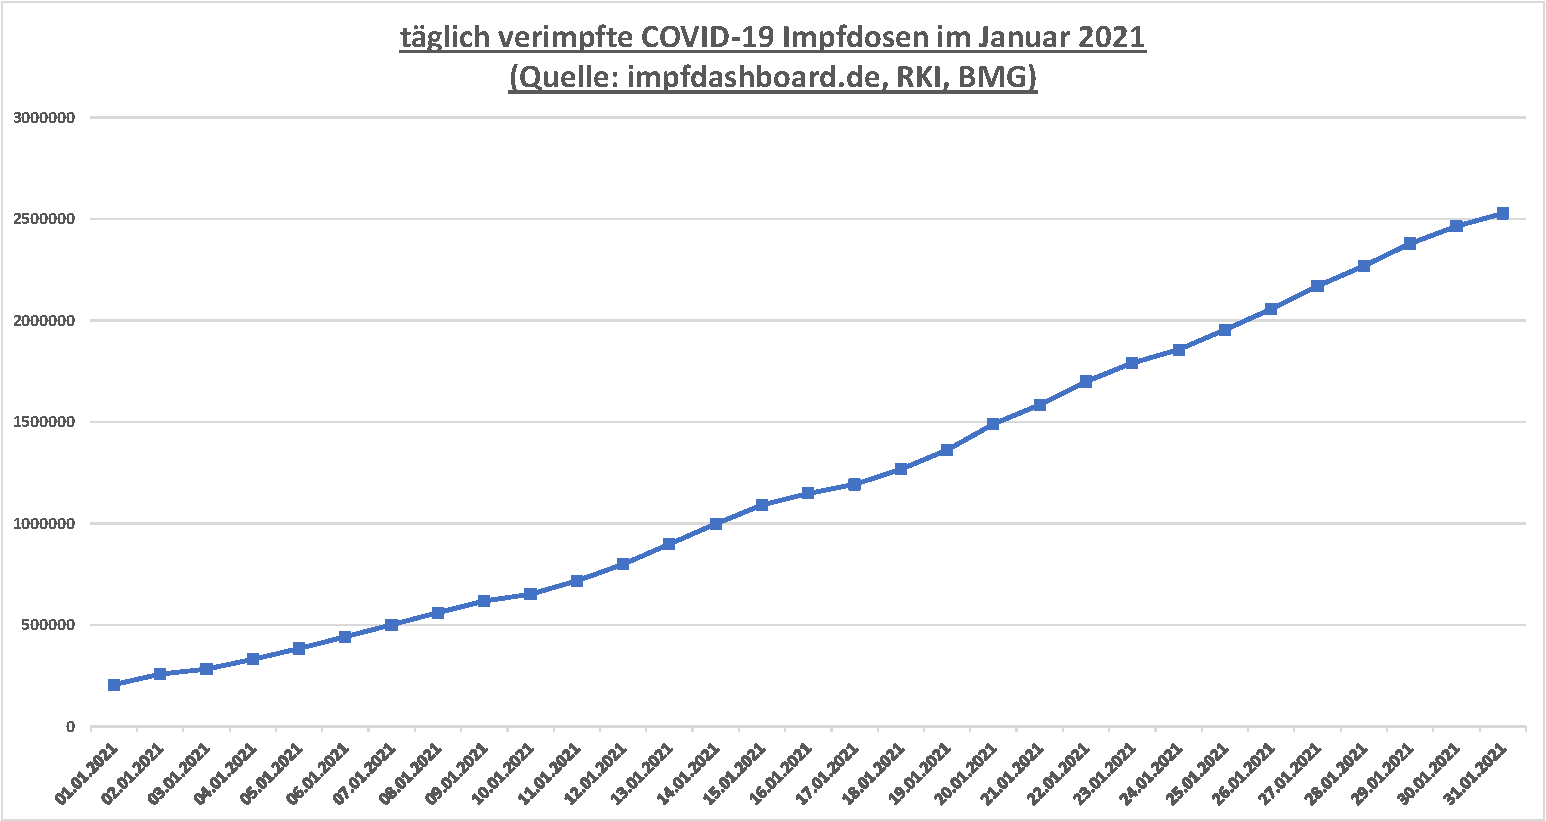
\includegraphics[width=\textwidth]{graphics/Beispiel-Zeitreihe.pdf}
\caption{Beispielhafte Zeitreihe aus dem Januar 2021}
\label{abb:BeispielZeitreihe}
\end{figure}

Die möglichen Anwendungen in der Informatik sind ebenfalls vielzählig. So können über virtuelle oder physikalische Sensoren Messwerte, wie beispielsweise die CPU Auslastung eines gegebenen Servers über die Zeit oder Temperaturmessungen eines \ac{IoT} Gerätes über die Zeit gemacht und gespeichert werden.

Ein wichtiges Merkmal von Zeitreihen ist die Distanz zwischen den Messwerten, im Sinne der Messfrequenz, in welcher Daten betrachtet werden. \Todo{belegen} Ist eine Zeitreihe äquidistant, wurde mit gleichbleibender Frequenz gemessen und die zeitliche Distanz zwischen einzelnen Messwerten ist gleich. Für die in dieser Arbeit diskutierten Auswertungsarten wird eine Äquidistanz der gemessenen Daten angenommen, da andernfalls ein Bias bei der Analyse nicht ausgeschlossen werden kann. Gleichfalls ist es technisch möglich einzelne, nicht äquidistante Messwerte auszusortieren. Die in \autoref{abb:BeispielZeitreihe} abgebildete Zeitreihe ist äquidistant, da die Werte einmal am Tag gesammelt erhoben wurden.


\Todo{Definition Zeitreihendaten}
\Todo{Definition Datenanalyse}

Bei der Verarbeitung von Daten ist zu beachten, dass der Wert, bzw. die Erkentnisse die aus den Daten abgleitet werden können, über die Zeit reduziert wird. \footcite[Vgl. auch im Folgenden][]{NucleusResarchInc..2012} In einer Analyse, die in \autoref{abb:DataHalflife} dargestellt wird, erhob Nucleus Research die Zahl, dass Daten für taktische Entscheidende nach maximal 30 Minuten die Hälfte des Wertes eingebüßt hat. Für operative Entscheidende ist die durchschnittliche Halbwertszeit nach acht Stunden erreicht, für strategische Entscheidende nach ca. 56 Stunden, also nach über 2 Tagen.
\begin{figure}[H]
\centering
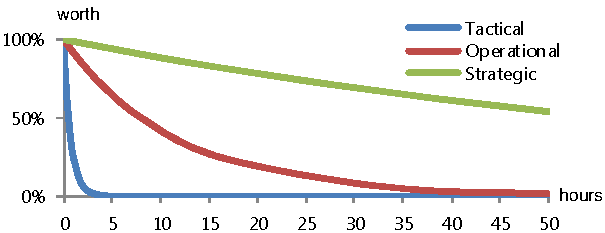
\includegraphics[width=\textwidth]{graphics/half-life-data.pdf}
\caption[Die Halbwertszeit von Daten]{Die Halbwertszeit von Daten\footnotemark}
\label{abb:DataHalflife}
\end{figure}
\footnotetext{Entnommen aus: \cite{NucleusResarchInc..2012}}
Aus diesen abweichenden Halbwertszeiten und damit aus den abweichenden Zeiträumen, in denen die erhobenen Daten den höchsten Wert haben, ergibt sich die Notwendigkeit von verschiedenen Datenverarbeitungsstrategien, um entsprechend strategischen, taktischen und operativen Entscheidenden die werthaltigsten Daten als Entscheidungsgrundlage zu präsentieren.



% \Todo{Grafik Data Analytics Pipeline}
\begin{figure}[H]
\centering
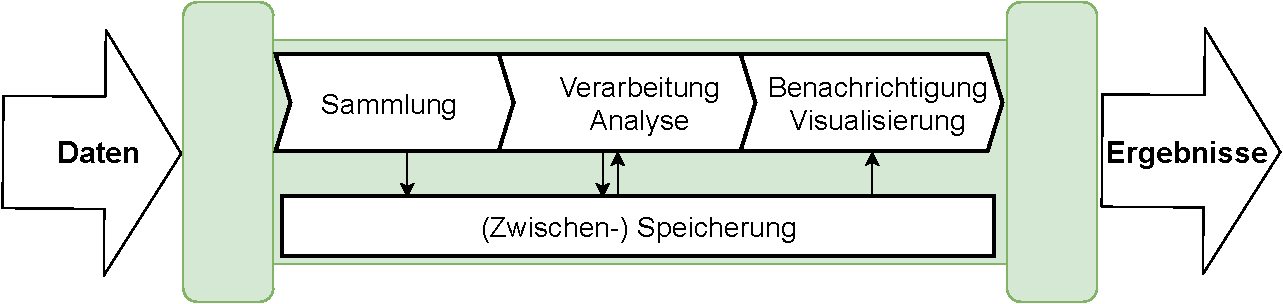
\includegraphics[width=\textwidth]{graphics/DataPipeline.pdf}
\caption{Aufbau und Ablauf in einer Data Pipeline}
\label{abb:DataPipeline}
\end{figure}
\Todo{Quellenangabe}


\subsection{Bestehende Referenzarchitekturkategorien}
Im Bereich der Streamingarchitekturen gibt es bereits etabblierte Referenzarchitekturen, welche verschiedene mögliche Aufbauarten einer Verarbeitung von Streaming/Zeitseriendaten zeigen.

% \Todo{Lambda, Kappa, OLAP elaborieren}
\begin{figure}[H]
\centering
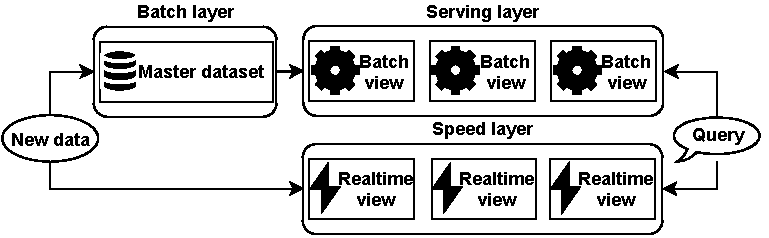
\includegraphics[width=\textwidth]{graphics/Lambda-Reference-Architecture.pdf}
\caption[$\lambda$-Datenstreaming Referenzarchitetktur]{$\lambda$-Datenstreaming Referenzarchitetktur.\footnotemark}
\label{abb:LambdaStreaming}
\end{figure}
\footnotetext{Mit Änderungen entnommen aus: \cite[][28]{Marz.2015}}
% Lambda nach \citeauthor{Marz.2015}, siehe \footcite[Vgl.][28]{Marz.2015}

Die von \citeauthor{Marz.2015} vorgestellte $\lambda$/Lambda-Architektur, welche in \autoref{abb:LambdaStreaming} gezeigt wird ist dabei eine der sehr bekannten Referenzarchitekturen. Der Name ist dabei nicht mit dem \ac{AWS} Dienst Lambda zu verwechseln, sondern ist wohl auf den gedrehten Buchstaben $\lambda$ zurückzuführen, also \reflectbox{\rotatebox[origin=c]{270}{$\lambda$}}.\footcite[Vgl. auch im Folgenden][]{Berle.27.11.2017} Die $\lambda$-Architektur sieht ausgehend von den hereingeladenen Daten zwei verschiedene Wege für die Daten vor. Zum einen den \enquote{Speed Layer}, welcher Daten direkt nach Eingang verarbeitet und nicht im Layer selbst speichert, sondern nur Aggregate oder Ergebnisse zur Verfügung stellt. Zum anderen gibt es den \enquote{Batch layer}, in welchem Daten zuerst in einem Master dataset gespeichert werden und dann in einem festen Intervall (\enquote{Batch jobs}) ausgewertet werden. Verschiedene Datenverarbeitungsintervalle machen speziell im Sinne der verschiedenen, in \autoref{abb:DataHalflife} gezeigten, Datenhalbwertszeiten Sinn. So sind manche Auswertungen, die präzise historische Daten benötigen in einem Batch layer besser möglich als in einem speed layer. Der speed layer bietet dagegen durch die Geschwindigkeit der Auswertungen die möglichkeit, agil auf erkannte Ereignisse oder Veränderungen im generellen zu reagieren.


\begin{figure}[H]
\centering
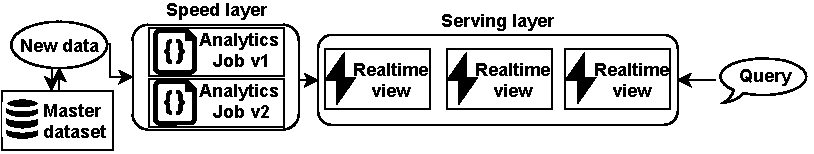
\includegraphics[width=\textwidth]{graphics/Kappa-Reference-Architecture.pdf}
\caption[$\kappa$-Datenstreaming Referenzarchitetktur]{$\kappa$-Datenstreaming Referenzarchitetktur.\footnotemark}
\label{abb:KappaStreaming}
\end{figure}
\footnotetext{Mit Änderungen entnommen aus: \cite{Kreps.2014}, \cite{Berle.27.11.2017}}

Die $\kappa$/Kappa Referenzarchitektur von \citeauthor{Kreps.2014}, dargestellt in \autoref{abb:KappaStreaming} basiert auf der $\lambda$-Architektur, spart jedoch den \enquote{Batch layer} mit zugehörigen \enquote{Batch jobs} aus. Das Konzept von Master Data existiert dabei weiterhin, jedoch in Form von Nachrichten, die in einem Messagebroker gespeichert werden. Analysen werden in Form von einzelnen, unveränderlichen Jobs über die vorhandenen Nachrichten erstellt. Wird die Analyse in irgendeiner Weise verändert (z.B. durtch Codeanpassungen) werden alle zwischengespeicherten Nachrichten erneut durch eine neue, unveränderliche Version des Jobs analysiert. Diese Unveränderlichkeit hat den Vorteil, dass keine unerwünschten Seiteneffekte durch Analysen, die gegenseitig Ergebnisse überschreiben auftreten. \Todo{elaborate on original source}

% Kappa nach \citeauthor{Kreps.2014},
% siehe \footcite[Vgl.][]{Kreps.2014}



\begin{figure}[H]
\centering
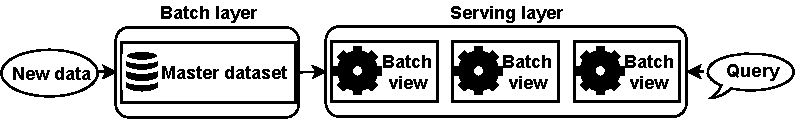
\includegraphics[width=\textwidth]{graphics/OLAP-Reference-Architecture.pdf}
\caption[OLAP Referenzarchitetktur]{OLAP Referenzarchitetktur.\footnotemark}
\label{abb:OLAPStreaming}
\end{figure}
\footnotetext{Mit Änderungen entnommen aus: \cite{Kreps.2014}}

%\ac{OLAP}
Aus der $\lambda$ Referenzarchitektur lässt sich auch eine, zur $\kappa$ Architektur gegenteilige Architektur aufzeigen, welche ein klassisches \ac{OLAP} Szenario aufzeigt. \Todo{Codd zitieren} Diese Architektur basiert, wie in \autoref{abb:OLAPStreaming} gezeigt, auf einer periodischen Verarbeitung der Daten im Master dataset. Dieses Vorgehen ist bei traditionellen Analytics weit verbreitet, bietet jedoch womöglich wichtige Einsichten erst nachdem die Datenhalbwertszeit bereits überschritten wurde.


\subsection{Arten der Auswertung}
\subsubsection{Median}
\subsubsection{Anomaliedetektion}
\subsubsection{Schwellwertüberschreitung}
\subsubsection{Trenderkennung/gleitender Durchschnitt}


\subsection{Echtzeitverarbeitung}
Gemäß der in \autoref{abb:KappaStreaming} gezeigten $\kappa$-Architektur gibt es Nutzungsfälle, in welchen eine reine Echtzeitauswertung basierend auf einer Datenquelle, wie beispielsweise dem Messagebroker Sinn machen kann. \citeauthor{Belur.2020} sieht dabei vier verschiedene Verwendungszwecke, in welchen die niedrige Verarbeitungslatenz besonders wichtig ist und den maximalen Wert aus den Daten zieht.\footcite[Vgl. auch im Folgenden][]{Belur.2020} Durch Echtzeit reporting und die Erstellung von Dashboards können aktuelle Daten schnell übersichtlich aufbereitet werden. Mittels erstellter Regeln, die Schwellwertüberschreitungen und Anomalien detektieren, können Nutzende benachrichtigt werden, sobald es zu einer Abweichung kommt. Ebenfalls sinnvoll ist Machine Learning zum auffinden von Mustern in den Daten zu verwenden, was verbesserte Anomalierkennung, Vorraussagen und ähnliche Features ermöglicht. Ein weiterer valider Usecase der $\kappa$-Architektur ist die Transformation von Daten in gewisse Zielformate, um beispielsweise Drittsysteme anzusprechen.
Requirements:
\begin{itemize}
\item Unified experience for data ingestion and edge processing
\item Versatile out-of-the-box connectivity
\item Scalable stream processing with complex transformations
\item Operationalized business rules and ML models
\item Ability to handle unstructured data and schema drift:
\item Reusability of processing logic
\item Governance and lineage
\end{itemize}

% \subsubsection{Streamanalyse}
% \begin{itemize}
% \item AWS Kinesis Data Analytics/Stream
% \item AWS Lambda
% \end{itemize}

\subsection{Datenbankseitige Verarbeitung}
\subsubsection{Datenbankabfragen}
\begin{itemize}
\item Timestream
\item Redshift
\item Athena
\item Elasticsearch
\end{itemize}

\subsubsection{Externe Analyse}
\begin{itemize}
\item Amazon EMR
\item Amazon Glue
\item AWS Lake Formation
\end{itemize}




Source -> Stream ingestion -> Stream storage -> Stream processing -> Destination

Talkingpoints gegen Streaming onprem:
Difficult to set up, Difficult to achieve high availability,
Error prone and complex to manage,
Tricky to scale, Integration requires development,Expensive to maintain

Amazon Kinesis Data Streams - Daten verfügbar in 70 Milisekunden



Amazon Kinesis Data Analytics


\subsubsection{Brokeranalyse}

\begin{itemize}
\item AWS IoT Analytics
\end{itemize}

\section{Referenzmodellierung}

\section{Theorie der Anforderungserhebung}



\section{Vergleichsmethodik für die Produktauswahl}\label{chap:vergleichsmethodik}

Desired properties of a Big Data system: \footcite[Vgl.][]{Marz.2015}
\begin{itemize}
\item Robustness and fault tolerance
\item Low latency reads and updates
\item Scalability
\item Generalization
\item Extensibility
\item Ad hoc queries
\item Minimal maintenance
\item Debuggability
\end{itemize}


\subsection{Featurevergleich}

\subsection{Performancevergleich}

\subsection{Kostenvergleich}




\chapter{Anwendung}

\section{Rahmenbedingungen der Datenverabeitung}\label{chap:rahmendatenverarbeitung}
Aufgrund bereits getroffener Architekturentscheidungen durch das \ac{IoT} Team der SPIRIT/21 GmbH wird für die Kommunikation zwischen Geräten und dem verarbeitenden Backend das \ac{MQTT} Protokoll verwendet. \ac{MQTT} ist nach eigener Aussage ein extrem leichtgewichtiges Standardprotokoll für publish-/subscribe-basierten Nachrichtentransport.\footcite[Vgl.][]{o.V..2020} Und ist nach Analystenmeinung der de-facto Standard für \ac{IoT} Kommunikation.\footcite[Vgl.][]{Skerrett.25.10.2019}\nzitat \footcite[Vgl.][]{Cabe.17.04.2018} 

In nachfolgenden Anwendungsfällen wird angenommen, dass eine technologische Vorauswahl für unterstützende AWS Dienste erfolgt ist.
So könnte beispielsweise ein beliebiger, \ac{MQTT} kompatibler Messagebroker eingesetzt werden, es wird jedoch davon ausgegangen, dass der eingesetzte Message Broker aus Kompatibilitätsgründen zu den anderen \ac{AWS} Diensten \ac{IoT} Core ist.



\section{Bestehende Anwendungsfälle}

\subsection{Luftqualitätssensoren}

\subsection{Raumbelegungsmonitoring}

\subsection{Sensor Simulator}\label{chap:iotdevicesim}
https://github.com/phyunsj/iot-device-simulator-1-mqtt
Mithilfe der Open Source
\begin{figure}[H]
\centering
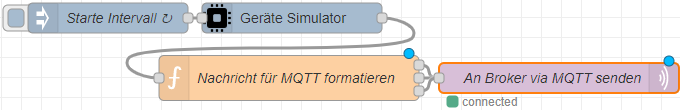
\includegraphics[width=\textwidth]{graphics/Device-Simulator-Flow.png}
\caption{Node-Red Flow des Sensorsimulators}
\label{abb:DeviceSimFlow}
\end{figure}




\section{Datenbankseitige Verarbeitung}



\section{Echtzeitverarbeitung}

\subsection{Auswahl eines geeigneten Produktes}

\subsubsection{AWS IoT Analytics}

\subsubsection{AWS Kinesis}

\subsubsection{AWS Lambda}

\subsection{Referenzmodellierung}

\section{Einsatzszenarien der Referenzmodelle}






\chapter{Produktauswahl}
Im nachfolgenden Kapitel werden mittels der in \autoref{chap:vergleichsmethodik} vorgestellten Methodik die Produkte für die finalen Referenzarchitekturen unter den in \autoref{chap:rahmendatenverarbeitung} vorgestellten Rahmenbedingungen verglichen und ausgewählt.

\section{Produkte für Echtzeitverarbeitung}\label{produkte:echtzeit}

\begin{figure}[H]
\centering
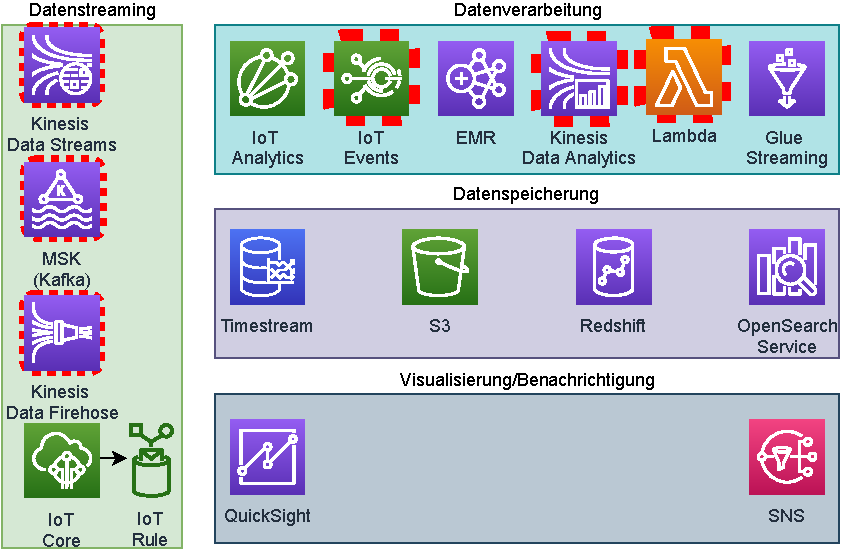
\includegraphics[width=\textwidth]{graphics/Overview-Realtime.pdf}
\caption{Einsetzbare Produkte im Bereich Echtzeitverarbeitung}
\label{abb:ProdukteRT}
\end{figure}


===========

Innerhalb des \ac{IoT} Core Brokers ist es möglich, Regeln zu definieren, die einzelne Nachrichten aus Topics in andere Dienste weiterzuleiten. Dazu müssen besagte Nachrichten selektiert werden, was mittels eines SQL Dialekts möglich ist. Eine beispielhafte Selektion könnte folgendermaßen aussehen: 


\begin{figure}[H]
\centering
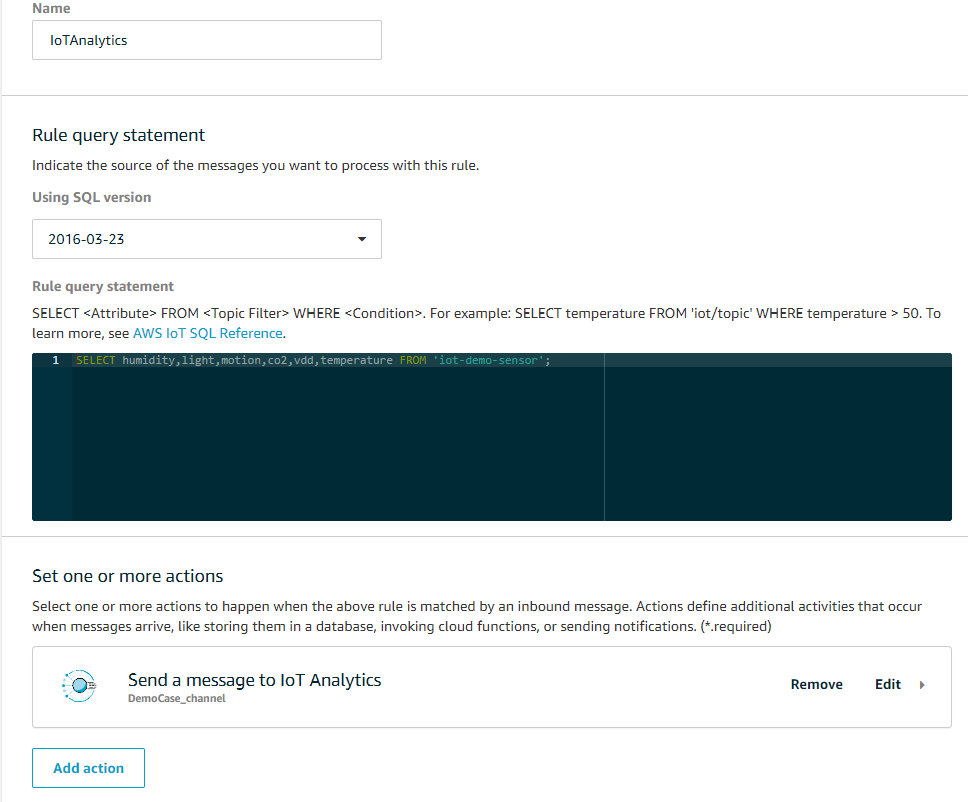
\includegraphics[width=\textwidth]{graphics/IoT-Rules-console.png}
\caption{Einstellung einer neuen Regel zur Weiterleitung an IoT Analytics}
\label{abb:IoTRulesExample}
\end{figure}

In \autoref{abb:IoTRulesExample} ist die Erstellung einer Weiterleitungsregel mit folgendem SQL Code zu sehen:
\lstset{language=SQL} 
\begin{lstlisting}
SELECT humidity,light,motion,co2,vdd,temperature 
FROM 'iot-demo-sensor'
\end{lstlisting}
Die Nachrichten aus dem Topic iot-demo-sensor werden dabei beispielhaft an IoT Analytics weitergeleitet.

\subsection{AWS IoT Analytics} \label{productselection:iotanalytics}
\AWSIOT Analytics ist ein Dienst der \AWSIOT Produktfamilie, der nach Aussage des Herstellers weitreichende Analysen von \ac{IoT} Daten, die beispielsweise via \AWSIOT Core geladen werden können, zulässt.
\begin{figure}[H]
\centering
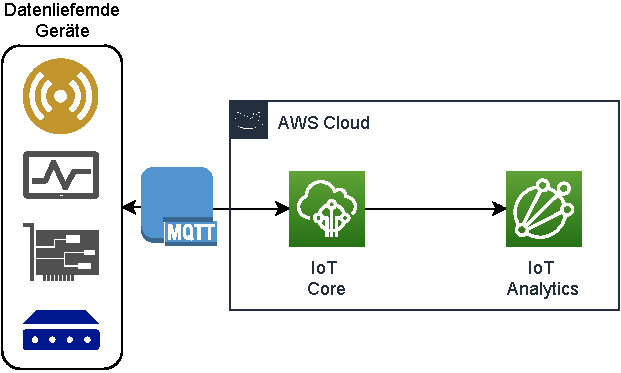
\includegraphics[width=0.8\textwidth]{graphics/IoT-Analytics-general.pdf}
\caption{Grobarchitektur des Ablaufes für IoT Analytics}
\label{abb:GrobArchitekturIoTAnalytics}
\end{figure}
In \autoref{abb:GrobArchitekturIoTAnalytics} ist die Grobarchitektur und Verknüpfung mit anderen Diensten unter Annahme der Vorraussetzungen aus \autoref{chap:rahmendatenverarbeitung} gezeigt. Datenliefernde Geräte, wie beispielsweise Sensoren liefern Zeitreihen-Messwerte via dem \ac{MQTT} Protokoll an. Die Weiterleitung zu IoT Analytics erfolgt mittels einer eingerichteten Regel im \ac{IoT} Core Messagebroker, welche mittels eines Dialekts der SQL Sprache gewisse Topics vorselektiert oder alle Topics zulässt.

\subsection{AWS IoT Events}

\begin{figure}[H]
\centering
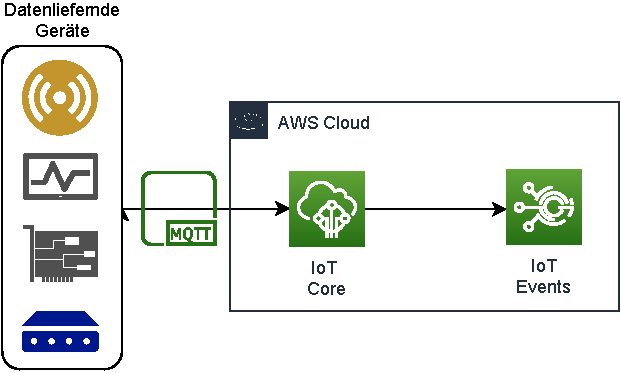
\includegraphics[width=0.8\textwidth]{graphics/IoT-Events-general.pdf}
\caption{Grobarchitektur des Ablaufes für IoT Events}
\label{abb:GrobArchitekturIoTEvents}
\end{figure}

\Todo{IoT Events ansprechen (Schwellwerte)}

\subsection{Amazon Kinesis}
Amazon Kinesis ist im Gegensatz zu \AWSIOT Analytics nicht allein auf die Analyse von \ac{IoT} Daten spezialisiert. Kinesis eignet sich vielmehr für generelle Analysen von allerlei Streamingdaten. Zusätzlich ist Amazon Kinesis älter als \AWSIOT Analytics.

\begin{figure}[H]
\centering
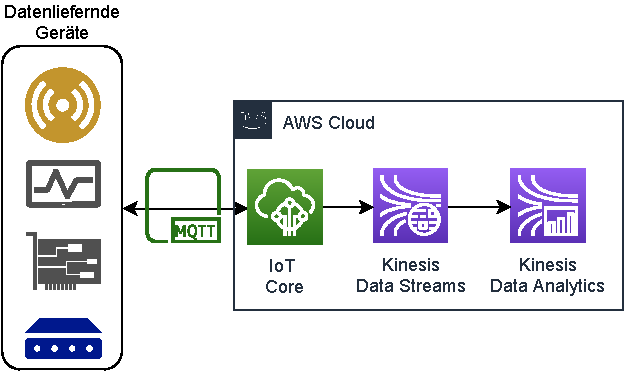
\includegraphics[width=0.8\textwidth]{graphics/Kinesis-Analytics-general.pdf}
\caption{Grobarchitektur des Ablaufes für Kinesis Analytics}
\label{abb:GrobArchitekturKinesisAnalytics}
\end{figure}
In \autoref{abb:GrobArchitekturKinesisAnalytics} ist das Zusammenspiel der Dienste aus der Kinesis Familie mit anderen Diensten dargestellt. Angenommen werden dabei die in \autoref{chap:rahmendatenverarbeitung} erläuterten Rahmenbedingungen, weshalb \ac{IoT} Core als Message Broker eingesetzt ist. Wie in der in \autoref{productselection:iotanalytics} beschriebenen Architektur, muss auch hier für die Datenverarbeitung eine Regel im \ac{IoT} Core Broker angelegt werden, um relevante Nachrichten an Kinesis Data Streams weiterzuleiten.\footcite[Vgl.][]{AmazonWebServicesInc..o.J.}

\begin{figure}[H]
\centering
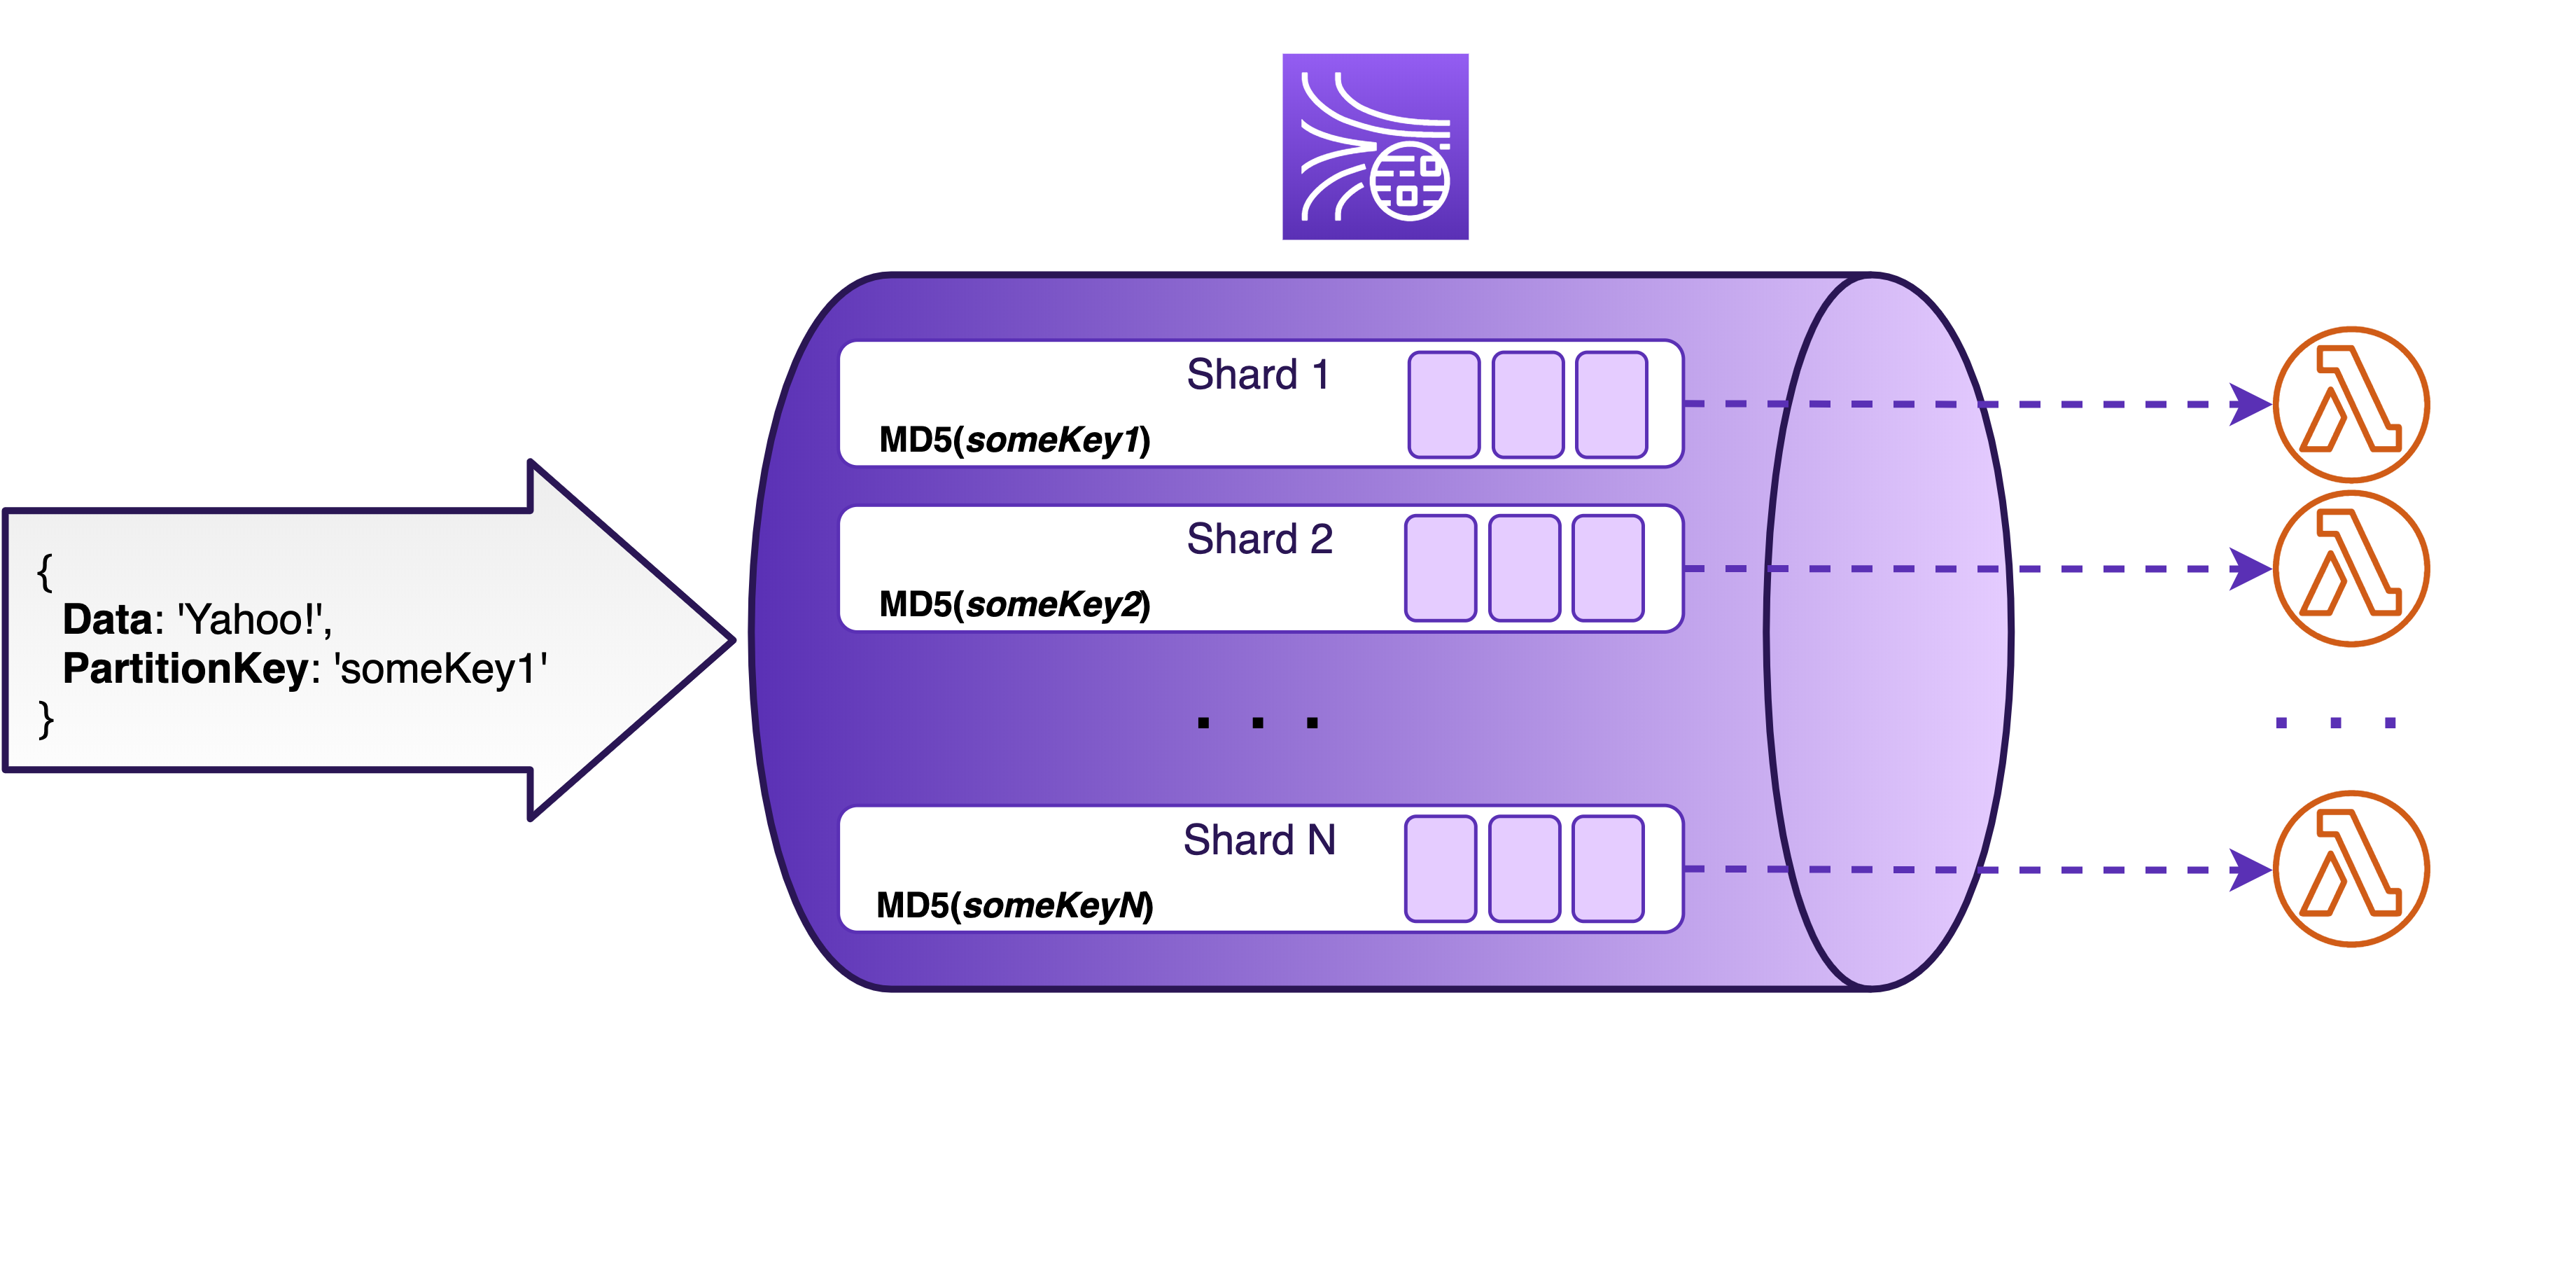
\includegraphics[width=\textwidth]{graphics/kinesis-inner-workings.png}
\caption[Funktionsweise von Kinesis]{Funktionsweise von Kinesis.\footnotemark}
\label{abb:KinesisShards}
\end{figure}
\footnotetext{Entnommen aus: \cite{Pogosova.28.05.2020}}
Kinesis unterteilt, wie in \autoref{abb:KinesisShards} gezeigt, Daten in einzelne Partitionen/Shards, in denen gleich partitionierte Datensätze verarbeitet werden können.\footcite[Vgl. auch im Folgenden][]{Pogosova.28.05.2020} Einzelne Shards verhalten sich dabei wie geordnete Warteschlangen und speichern die Nachrichten nach Eingangsdatum sortiert. 


\subsection{AWS Lambda}
Bei \ac{AWS} Lambda handelt es sich um die Amazon Implementierung eines \ac{FaaS} Dienstes. Innerhalb dieser Arbeit wird Lambda als einzige generelle Computing Plattform betrachtet, da Alternativen wie \ac{EC2}, welches virtuelle Maschinen anbietet oder \ac{ECS}, welches Container anbietet einen von einzelnen Events unabhängigen Lebenszyklus haben. So laufen Container auf \ac{ECS} oder virtuelle Maschinen auf \ac{EC2}, wenn nicht anders konfiguriert kontinuierlich und holen/ \enquote{fetchen} Daten. In Zeiträumen, in denen keine Daten bereitstehen sind die entsprechenden Container und virtuellen Maschinen im Leerlauf, was unnötige Kosten erzeugt. Lambda hingegen wird von unterstützenden Diensten zur Verarbeitung von Events aufgerufen. Dabei ist je nach Dienst einstellbar, ob ein Aufruf pro Event stattfinden soll, oder Events zu einer konfigurierbaren Anzahl gruppiert werden und dann an Lambda übergeben werden. Lambda eignet sich besonders für analytische Workloads, seit der kürzlichen Addition von Intels \ac{AVX2}, einem speziellen CPU-Instruktionssatz, der die Verarbeitung von Vektorinstruktionen, wie sie beispielsweise beim Machine Learning oder in der Statistik vorkommen, beschleunigt.\footcite[Vgl.][]{Beswick.24.11.2020} Aufgrund der zentralen Rolle im Bereich Compute bei \ac{AWS}, können viele Dienste Events an Lambda senden. In \autoref{abb:GrobArchitekturLambda} sind als Integrationsbeispiele die \acp{MoM} \ac{IoT} Core, MQ und Kinesis Data Streams als Eventlieferanten gezeigt.
\begin{figure}[H]
\centering
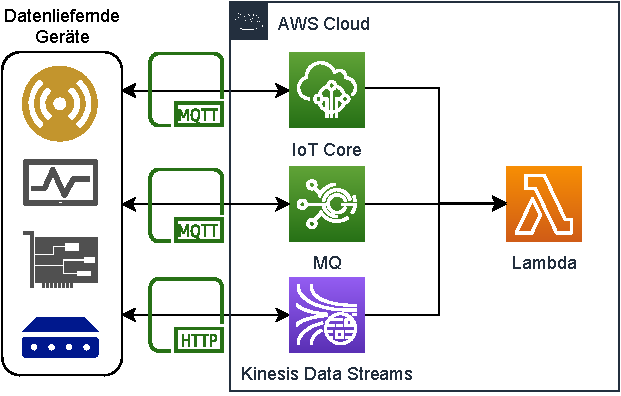
\includegraphics[width=0.8\textwidth]{graphics/Lambda-general.pdf}
\caption{Grobarchitektur des Ablaufes für Lambda}
\label{abb:GrobArchitekturLambda}
\end{figure}

\subsection{Amazon MSK}
Bei \ac{MSK} handelt es sich um einen Managed Service für die Open Source Lösung Apache Kafka. Im Gegensatz zu anderen, hier im Kapitel aufgeführten Lösungen wie \ac{IoT} Analytics, hat Amazon \ac{MSK} nicht von Grund auf selber entwickelt, sondern einen großen Teil des Codes von Apache Kafka übernommen. Dies erklärt auch, warum die Anbindung an andere Dienste von Amazon bedeutend schwieriger ist, als beispielsweise an \ac{IoT} Core. In der in \autoref{abb:GrobArchitekturMSK} abgebildeten Grobarchitektur müsste zur Anbindung von Apache Kafka an zuliefernde Geräte ein Intermediär wie \ac{IoT} Core verrwendet werden, da Apache Kafka ein eigenes, binäres Protokoll hat, welches sonst in die Geräte implementiert werden müsste. \Todo{letzten Halbsatz belegen} Umgangen kann die Implementierung des Kafka Protokolls auf dreierlei Arten: Zum einen lassen sich mittels Kafka Connect for \ac{MQTT} \ac{MQTT} Broker als Eventquellen anbinden.\footcite[Vgl.][]{Erber.12.01.2021} Alternativ kann Kafka auch als \ac{MQTT} Proxy dienen, was bedeutet, dass Kafka als eigenständiger MQTT Broker agiert, wobei zu beachten ist, dass Kafka weit nicht alle \ac{MQTT} Standardelemente implementiert und eine paralelle Weiterverarbeitung in anderen Amazon Diensten nicht möglich ist.\footcite[Vgl.][]{Erber.12.01.2021} Zuletzt gibt es noch die Möglichkeiten, die Nachrichten via \ac{IoT} Core innerhalb von \ac{AWS} an \ac{MSK} weiterzuleiten, was auch in \autoref{abb:GrobArchitekturMSK} dargestellt ist.
\begin{figure}[H]
\centering
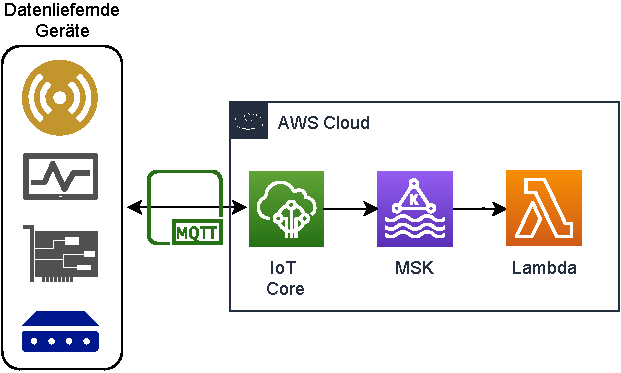
\includegraphics[width=0.8\textwidth]{graphics/MSK-general.pdf}
\caption{Grobarchitektur des Ablaufes für Managed Streaming for Apache Kafka}
\label{abb:GrobArchitekturMSK}
\end{figure}

Kafka hat eigene Verarbeitungslogiken integriert, mit welchen einige Analysen bereits durchgeführt werden können. Um diese in \ac{AWS} weiterverarbeiten zu können, müssen die Ergebnisse via der Integration mit Lambda oder der Integration mit \ac{EC2}, der Amazon Plattform für virtuelle Maschinen abgerufen werden.

=> binary protocol no \ac{MQTT} Support, redundant, only Lambda and EC2 conenctivity

\subsection{Produktauswahl}

\section{Produkte für datenbankseitige Verarbeitung}

\subsection{Amazon Timestream}

\subsection{Amazon Redshift}

\subsection{Amazon Athena}

\subsection{Amazon Glue}

\subsection{Produktauswahl}

\chapter{Modellierung}
\section{Anforderungserhebung}
Wie in \autoref{theorie:referenzmodellierung} beschrieben, müssen Referenzmodelle einen subjektiven Empfehlungscharakter besitzen, damit sie akzeptiert und wiederverwendet werden. Dafür muss ein Abgleich mit den Anforderungen der Nutzenden geschehen. Um dies zu erreichen, wurden im Anhang transkribierte Interviews \Todo{Hier RM-Interviews verlinken} durchgeführt. Daraus ergeben sich folgende Anforderungen an die zu konstruierenden Referenzmodelle:
\Todo{Anforderungstabelle}
\section{Echtzeitverarbeitung}

\section{Datenbankseitige Verarbeitung}

\section{Einsatzszenarien der Referenzmodelle}


\chapter{Schlussbetrachtung}

\section{Fazit}

\section{Handlungsempfehlung}

\section{Ausblick}

\clearpage
\todos
%\chapter{Einleitung}

% \chapter{Zitieren}\label{chapter:zitate}

Der Zitierstil ist so angepasst, dass er den Zitierrichtlinien des Studiengangs Wirtschaftsinformatik der DHBW Stuttgart entspricht. 

\section{Zitate in den Text einfügen}
In \LaTeX\ wird mit den Befehlen \verb|\footcite| 
oder 
\verb|\cite|
eine Referenz im Text eingefügt. Meist wird \verb|\cite| nur \emph{innerhalb} einer Fußnote benutzt. 
Damit ein vorangestelltes \enquote{Vgl.} in der Fußnote erscheint, können Sie wie folgt zitieren:
\begin{verbatim}
\footcite[Vgl.][S. 3]{Autor}
\footcite[Vgl.][]{Autor}
\end{verbatim}

Das erste optionale Argument von \verb|\footcite| wird dem Zitat vorangestellt, das zweite ist die Seitenzahl. Den selben Effekt hätte
\begin{verbatim}
\footnote{Vgl. \cite[S. 3]{Autor}}
\footnote{Vgl. \cite{Autor}}
\end{verbatim}

Hinweis: Falls \enquote{Vgl.}, aber keine Seitenzahl angeben werden soll, muss das zweite Argument vorhanden (jedoch leer) sein, ansonsten wird \enquote{Vgl.} als Seitenzahl interpretiert. Falsch ist also: 
\begin{verbatim}
\footcite[Vgl.]{Autor}  % so nicht!
\end{verbatim}



\subsection{Beispiele}
Nachfolgend ein paar Beispiele, um die korrekte Darstellung zu überprüfen:

\begin{itemize}
\item \cite{Schlosser} ist ein Buch über \LaTeX.
\item Zur Vorlesung \emph{Logik und Algebra} gibt es das gleichnamige Lehrbuch.\footcite{Staab}
\item nochmal dasselbe Buch\footcite{Staab}
\item ein weiteres Buch desselben Autors\footcite{BuschlingerStaab}

\item Der Konferenzbeitrag \cite{Ancuti} beschäftigt sich mit Bildverarbeitung.
\item Cloud Computing wird in einer Diplomarbeit erklärt.\footcite[S.~14]{Boettger:Diplomarbeit}
\item Preiß\footcite{Preiss} gibt eine Einführung in Datenbanken.
\item Eine Erläuterung, was \enquote{Intangibles} sind, findet sich bei Stoi\footcite[S.~82]{Stoi}.
\item weitere Ausführung in derselben Quelle\footcite[Vgl.][S.~84]{Stoi}
\item Laut Wikipedia\footcite[Abschnitt~5]{wiki:Wirtschaftsinformatik} ist Wirtschaftsinformatik ein interessantes Studienfach.
\item ITIL-Prozesse kann man tatsächlich auch mit \LaTeX\ dokumentieren.\footcite{Carvalho:PJ:2012-1}
\item Open-Source und Cloud-Computing in einem Buchbeitrag\footcite{Wind}
\item Buch mit zwei Autoren\footcite{MitZweiAutoren}
\item Buch mit drei Autoren\footcite{MitDreiAutoren}
\item Buch ohne Autor\footcite{OhneAutoren}
\item Buch ohne Autor und ohne Jahr\footcite{OhneAutorenOhneJahr}
\item und noch ein anderes Buch ohne Autor und ohne Jahr\footcite{OhneAutorenOhneJahr2}
\item Buch ohne Autor, aber dafür mit Herausgeber\footcite{keinAutorAberHerausgeber}

\item manche Bachelorarbeit baut auf einer vorhergehenden Projektarbeit\footcite{mayer:PA1} auf
\item das Handbuch zu BibLaTeX\footcite{biblatex:manual} und eines zu Windows 8\footcite{Win8}
\item zwei Beiträge zu Büchern\footcite{Trautwein:Nokia}${}^{,}$\footcite{Mann} und zu einem Konferenzband\footcite{Trautwein:Erfolgsfaktoren}
\item eine Online-Quelle\footcite{SAP:HANA}
\item eine plagiierte Dissertation,\footcite{GuttenPlag} nicht zur Nachahmung empfohlen
\item zum Testen, ob Umlaute und Sonderzeichen korrekt wiedergegeben werden\footcite{Umlauttest}
\end{itemize}

\subsection{Spezialfälle}
\begin{itemize}
\item \emph{Zwei Quellen am Satzende} werden durch Komma getrennt.\footcite{Staab}${}^{,}$\footcite{mayerLukas:PA1} Hier muss \verb|${}^{,}$| eingeschoben werden.
\item \emph{Eindeutigkeit:} Normalerweise wird kein Vorname des Autors angegeben. Falls es allerdings zur Eindeutigkeit\footnote{\cite{trautwein2011unternehmensplanspiele} vs. \cite{hitzler2011optimierung}} (bei gleicher Jahreszahl) erforderlich ist, wird der Vorname abgekürzt bzw.\ nötigenfalls sogar ganz ausgeschrieben mit angegeben.\footnote{Vgl. \cite{mayer:PA1} und \cite{mayerLukas:PA1}}
 
Welch ein Glück, dass Sie sich darum dank \LaTeX\ gar nicht kümmern müssen (arme Word\texttrademark-User ;-).

\item Die Verwendung von \emph{Sekundärliteratur}\footcitePrimaerSekundaer{Primaerquelle}{}{Sekundaerquelle}{11} wird weiter in Abschnitt~\ref{sec:sekundaerliteratur} erläutert.
\end{itemize}


\section{Eintragstypen für die Literatur-Datenbank}

Die verwendete Literatur pflegen Sie in einer Literatur-Datenbank im Bibtex-Format. Dabei handelt es sich um eine Textdatei, wobei für jede Quelle mittels Name-Value-Pairs die relevanten Attribute (Autor, Titel etc.) hinterlegt sind. Die Datei wird üblicherweise nicht im Texteditor, sondern in einem spezialisierten Programm wie JabRef bearbeitet.

Sofern in der Literatur-Datenbank der Typ eines Eintrags (Entry Type) korrekt festgelegt ist, wird er im Literaturverzeichnis automatisch richtig dargestellt. Mit folgenden Typen sollten Sie i.d.R.\ auskommen:
\begin{description}
\item[article] Artikel in einer Fachzeitschrift, auch E-Journal (Zeitschrift in elektronischer Form)\footnote{Bei E-Journals/E-Books werden beim Zitieren anstelle der (u.U. nicht eindeutigen, da von der Schriftgröße abhängigen) Seitenzahl Abschnitt und Absatz näher bezeichnet, also: \cite[Abschnitt 1.2.3, Absatz 4]{Staab}.}
\item[book] Buch, auch E-Book 
\item[inbook] Kapitel in einem Buch, zu dem mehrere Autoren beigetragen haben 
\item[inproceedings] Beitrag zu einer Fachtagung/Konferenz 
\item[manual] Handbuch
\item[misc] anderweitig nicht zuordenbarer Typ
\item[phdthesis] Dissertation
\item[thesis] Bachelor-/Master-/Diplomarbeit (Art wird im Attribut \enquote{type} festgelegt) 
\item[online] Internet- oder Intranet-Quelle\footnote{\label{fn:onlineEntryType}Man beachte, dass der Eintragstyp \enquote{online} in JabRef nur im \enquote{biblatex-Modus} (Menü: Datei -- Neue biblatex Bibliothek) auswählbar ist.}
\item[report] technischer Bericht, Forschungsbericht oder White Paper; diesen Typ können Sie auch verwenden, um eine Projektarbeit zu zitieren (Art wird im Attribut \enquote{type} festgelegt) 
\end{description} 

Eine Übersicht über die notwendigen Attribute jedes Eintragstyps gibt die folgende Tabelle, wobei ein Schrägstrich als \enquote{oder} zu verstehen ist.\footnote{Auszugsweise entnommen aus \cite{biblatex:manual}.} Zudem sind die wichtigsten optionalen Attribute aufgeführt.

\begin{tabular}{l|p{6cm}|p{6cm}}
\textbf{Eintragstyp} & \textbf{notwendige Attribute} & \textbf{optionale Attribute (Auswahl)} \\
\hline
article & author, title, journal, year/date  & volume, number, pages, month, note \\
\hline
book & author, title, year/date  & publisher, edition, editor, \mbox{volume/number}, series, isbn, url \\
\hline
inbook & author, title, booktitle, year/date  & bookauthor, editor, volume/number, series, isbn, url \\
\hline
inproceedings & author, title, booktitle, year/date  & organization/publisher, editor, volume/number, series, isbn, url  \\
\hline
manual & author/editor, title, year/date  & organization/publisher, address, edition, month, note, url, urldate \\
\hline
misc & author/editor, title, year/date & howpublished, organization, month, note \\
\hline
phdthesis & author, title, institution, year/date  & address, month, note \\
\hline
thesis & author, title, institution, type, year/date &  address, month, note \\
\hline
online\textsuperscript{\ref{fn:onlineEntryType}} & author/editor, title, year\footnotemark/date, url & urldate \\
\hline
report & author, title, institution, type, year/date & number, version, url, urldate \\
\end{tabular}
\footnotetext{%
Sofern kein Jahr bekannt ist, sollte das Attribut nicht leer gelassen werden (sonst wird die aktuelle Jahreszahl automatisch eingefügt), sondern der Eintrag \enquote{o.J.} gewählt werden.}



\section{Zitieren von Sekundärliteratur}\label{sec:sekundaerliteratur}
Gelegentlich lässt es sich nicht vermeiden, aus der Sekundärliteratur zu zitieren. Dies leistet der folgende Befehl.
\begin{verbatim}
\footcitePrimaerSekundaer{Primaerquelle}{Seite}{Sekundaerquelle}{Seite}
\end{verbatim}
Die erste Seitenangabe bezieht sich auf die Primär-, die zweite auf die Sekundärquelle.
Die Seitenangaben sind optional, sie können auch leer bleiben.\footcitePrimaerSekundaer{Primaerquelle}{23}{Sekundaerquelle}{}
Es ist aber zu beachten, dass der Befehl \verb|\footcitePrimaerSekundaer| vier Argumente hat.

Ins Literaturverzeichnis soll nur die Sekundärquelle aufgenommen werden. Dies wird dadurch erreicht, dass in der Literatur-Datenbank bei der Primärquelle im Attribut \enquote{keyword} der Wert \enquote{ausblenden} eintragen wird.

% \chapter{Beispiele für Abbildungen und Tabellen}\label{chapter:abbildungenTabellen}

Hier finden Sie Beispiele für Abbildungen, Tabellen, Formelsatz und  Source Code.

\section{Abbildungen}
In diesem Abschnitt gibt die Abbildungen~\ref{abb:Logo2cmHoch} und~\ref{abb:Logo2cmBreit}, die beide das Logo der DHBW zeigen.

\begin{figure}[H]
\centering

\includegraphics[height=2cm]{graphics/dhbw.png}
\caption[DHBW-Logo 2cm hoch]{DHBW-Logo 2cm hoch.\footnotemark}
\label{abb:Logo2cmHoch}
\end{figure}
\footnotetext{Mit Änderungen entnommen aus: \cite{OhneAutorenOhneJahr}}

\lstset{language=TeX, % hervorzuhebende Keywords definieren
  morekeywords={footnotetext,footnotemark,footcite,caption}
}

\emph{Spezialfall:} Sofern \emph{innerhalb} der Bezeichnung einer Abbildung eine Fußnote angegeben oder eine Quelle referenziert werden soll, geschieht dies nicht per \lstinline|\footnote| oder \lstinline
|\footcite|. Vielmehr sind die Befehle \lstinline|\footnotemark| und \lstinline|\footnotetext| zu verwenden und außerdem das optionale Argument für \lstinline|\caption| anzugeben (vgl.\ Source Code).

\begin{figure}[htb]
\centering

\includegraphics[width=2cm]{graphics/dhbw.png}
\caption[DHBW-Logo 2cm breit.]{DHBW-Logo 2cm breit. (Quelle: DHBW\footnotemark)}
\label{abb:Logo2cmBreit}
\end{figure}
\footnotetext{\url{www.dhbw.de}}



\section{Tabellen}

In diesem Abschnitt gibt es zwei Beispiel-Tabellen, nämlich auf Seite~\pageref{tab:BeispielTabelleKlein} und auf Seite~\pageref{tab:BeispielTabelleGroesser}.

\begin{table}[htb]
\centering
\begin{tabular}{lcr}
links & Mitte & rechts \\
\hline
Muster & Muster & Muster \\
\end{tabular}
\caption{Kleine Beispiel-Tabelle.}
\label{tab:BeispielTabelleKlein}
\end{table}

\begin{table}[htb]
\centering
\begin{tabular}{|l|l|c|l|r||l}
    \textbf{Spalte 1} & \textbf{Spalte 2} & \textbf{Spalte 3} & \textbf{Spalte 4} & \textbf{Spalte 5} & \textbf{Spalte 6} \\
    \hline
    a        & b          & c                & d        & e        & f        \\
    Test     & Test, Test & Test, Test, Test & ~        & ~        & ~        \\
    1        & 2          & 3                & 4        & 5        & 6        \\
\end{tabular}
\caption{Größere Beispiel-Tabelle.}
\label{tab:BeispielTabelleGroesser}
\end{table}

\section{Etwas Mathematik}

Eine abgesetzte Formel:
\[
  \int_a^b x^2 \: \mathrm{d} x = \frac{1}{3} (b^3 - a^3)
\]

Es ist $a^2+b^2 = c^2$ eine Formel im Text.

\section{Source Code}

Source Code-Blöcke können auf folgende Arten eingefügt werden:

\lstset{language=Java}

Direkt im \LaTeX-Source Code:
\begin{lstlisting}
if(1 > 0) {
  System.out.println("OK"); 
} else {
  System.out.println("merkwuerdig");
}
\end{lstlisting}

oder eingefügt aus einer externen Datei.
\lstinputlisting{includes/HelloWorld.java}

% \chapter*{Anhang}
\addcontentsline{toc}{chapter}{Anhang}
\section*{Anhangverzeichnis}
\vspace{-8em}

% vor \listofanhang müssen Einrückungen angepasst werden
\abstaendeanhangverzeichnis

\listofanhang
\clearpage
\spezialkopfzeile{Anhang} % damit in der Kopfzeile das Wort "Anhang" angezeigt wird

\anhang{So funktioniert's}

\lstset{language=TeX, % hervorzuhebende Keywords definieren
  morekeywords={anhang, anhangteil}
}



% \anhangteil{Wieder mal eine Abbildung}\label{anhang:abbildung}
% \begin{figure}[htb]
% \centering
% 
\includegraphics[width=0.9\linewidth]{graphics/dhbw.png}
% \caption{Mal wieder das DHBW-Logo.}
% \end{figure}

% \anhangteil{Etwas Source Code}\label{anhang:sourcecode}
% \lstinputlisting{includes/HelloWorld.java}


% \anhang{Release Notes}
\anhangteil{Änderungen in Version 1.1}\label{anhang:ReleaseNotes11}
In Version 1.1 sind einige Rückmeldungen, die nach der Einführungsvorlesung am 6.2.2015 oder nach Veröffentlichung der Vorlage in Moodle eingegangen sind, berücksichtigt worden. Korrekturen sind mit \enquote{(Fix)} gekennzeichnet. 

\begin{itemize}
\item \verb|latex-vorlage.tex|
\begin{itemize}
\item (Fix) Abkürzungsverzeichnis wird vor Abbildungsverzeichnis platziert
\item (Fix) Abbildungs- und Tabellenverzeichnis in Inhaltsverzeichnis aufgenommen
\item (Fix) Quellenverzeichnis wird nun ohne Kapitelnummer dargestellt

\item eingebundene Dateien in Unterverzeichnissen \verb|includes| bzw.\ \verb|graphics|
\item Beispiel-Anhang (Datei \verb|anhang.tex|) mit Erklärungen wurde eingebunden 
\end{itemize}

\item \verb|_dhbw_praeambel.tex|
\begin{itemize}
\item (Fix) das Paket hyperref wird nach biblatex eingebunden, um ein Problem mit der Verlinkung der Fußnoten im PDF zu beheben
\item (Fix) Fußnoten  gemäß der Richtlinien fortlaufend nummeriert und nicht pro Kapitel
\item Einstellungen hinzugefügt, um Anhangsverzeichnis zu ermöglichen
\item bessere Kompatibilität zwischen KOMA-Script (scrreprt) und anderen Paketen mittels scrhack
\end{itemize}

\item \verb|_dhbw_biblatex-config.tex|
\begin{itemize}
\item (Fix) keine Abschnittsnummern für einzelne Verzeichnisse im Quellenverzeichnis
\end{itemize}

\item \verb|abbildungen_und_tabellen.tex|
\begin{itemize}
\item Erklärung, wie eine Fußnote/ein Zitat bei einer Abbildung zu erstellen ist
\end{itemize}

\item \verb|abkuerzungen.tex|
\begin{itemize}
\item Abkürzungsverzeichnis wird im Inhaltsverzeichnis aufgeführt
\end{itemize}

\item \verb|abstract.tex|, \verb|anhang.tex|, \verb|einleitung.tex| 
\begin{itemize}
\item Erklärungen im Text ergänzt
\end{itemize}

\item \verb|deckblatt.tex|
\begin{itemize}
\item Meta-Daten (Autor, Titel) für die generierte PDF-Datei lassen sich nun festlegen
\end{itemize}

\end{itemize}


\anhangteil{Änderungen in Version 1.2}\label{anhang:ReleaseNotes12}
Über das Forum in Moodle sind einige Rückmeldungen eingegangen -- vielen Dank an alle, die dazu beigetragen haben. In der Version 1.2 wurden folgende Änderungen vorgenommen, wobei Korrekturen wieder mit \enquote{(Fix)} gekennzeichnet sind: 

\begin{itemize}
\item \verb|latex-vorlage.tex| (Hauptdokument)
\begin{itemize}
\item (Fix) Zeile 19: Seitenzahlen zu Beginn mit römischen \emph{Groß}buchstaben nummeriert
\end{itemize}

\item \verb|_dhbw_praeambel.tex|
\begin{itemize}
\item Zeile 39/40: Unterstützung für \enquote{ebenda} 
\item Zeile 46--68: zweite Gliederungsebene für Anhänge ermöglicht
\item (Fix) Zeile 70--73: Abbildungen und Tabellen: Zähler fortlaufend, kein Rücksetzen zu Kapitelbeginn (Paket \verb|chngcntr| anstelle von Paket \verb|remreset|)
\end{itemize}

\item \verb|_dhbw_biblatex-config.tex|
\begin{itemize}
\item (Fix) bei Quellen mit Herausgeber, aber ohne Autor wird der Name des Herausgebers im Verzeichnis fett gedruckt
\item Unterstützung für \enquote{ebenda} 
\end{itemize}

\item \verb|abkuerzungen.tex|
\begin{itemize}
\item Bemerkungen zur fortgeschrittenen Nutzung des \verb|acronym|-Pakets eingefügt 
\end{itemize}

\item \verb|einleitung.tex|
\begin{itemize}
\item Abschnitt 1.3 zu Einstellungen ergänzt
\item Abschnitt 1.5 zu Fehlerbehebungen eingefügt 
\end{itemize}

\item \verb|text-mit-zitaten.tex|
\begin{itemize}
\item Abschnitt 3.1 eingefügt, Erläuterungen zum Zitieren mit \enquote{vgl.} und \enquote{ebenda}. 
\item Abschnitt 3.2: Beispiele ergänzt
\item Hinweis zu Jahreszahlen bei Online-Quellen
\end{itemize}

\item \verb|anhang.tex|
\begin{itemize}
\item Erläuterungen zur zweiten Gliederungsebene
\end{itemize}

\item \verb|literatur-datenbank.bib|
\begin{itemize}
\item weitere Beispiele für Quellen
\end{itemize}

\end{itemize}

\anhangteil{Änderungen in Version 1.3}\label{anhang:ReleaseNotes13}
Durch die ab 1/2016 geltenden Änderungen der Zitierrichtlinien des Studiengangs waren einige kleinere Anpassungen der Vorlage erforderlich, die nachfolgend beschrieben sind. Bei dieser Gelegenheit ebenfalls erfolgte Korrekturen sind wieder mit \enquote{(Fix)} gekennzeichnet:

\begin{itemize}
\item \verb|latex-vorlage.tex| (Hauptdokument)
\begin{itemize}
\item Hinweis auf Option doppelseitiger Druck entfernt
\item Schriftgröße der Kapitelüberschriften verkleinert
\item (Fix) Kopf- und Fußzeilen werden nun korrekt angezeigt für erste Seite eines Kapitels und auch  Quellenverzeichnisse
\end{itemize}

\item \verb|_dhbw_praeambel.tex|
\begin{itemize}
\item Angabe des unteren Rands für Seitenzahl, da diese nun unten rechts steht
\item Unterstützung für \enquote{ebenda} entfernt
\item (Fix) Präfixe wie \enquote{von} im Namen eines Autors werden berücksichtigt
\item Anpassung der Abstände bei Kapitelüberschriften
\item Kopf- und Fußzeile für Verzeichnisse nun in \verb|_dhbw_kopfzeilen.tex| definiert 
\end{itemize}


\item \verb|deckblatt.tex|
\begin{itemize}
\item Schriftgröße des Titels vergrößert
\item Befehl \verb|\typMeinerArbeit| eingeführt, um Typ auszuwählen
\item Festlegung des Themas (für ehrenwörtliche Erklärung) mit Befehl \verb|\themaMeinerArbeit|
\item Darstellung der Angabe des Betreuers in der Ausbildungsstätte angepasst
\item Formulierung des Sperrvermerks angepasst  
\end{itemize}

\item \verb|_dhbw_erklaerung.tex|
\begin{itemize}
\item Formulierung angepasst an geänderte Prüfungsordnung
\item Typ und Thema der Arbeit werden automatisch eingefügt
\end{itemize}

\item \verb|_dhbw_kopfzeilen.tex|
\begin{itemize}
\item Seitennummern stehen jetzt unten rechts
\item (Fix) Kopf- und Fußzeile werden nun korrekt angezeigt in Verzeichnissen und dem Anhang
\end{itemize}

\item \verb|_dhbw_biblatex-config.tex|
\begin{itemize}
\item Anpassung des Zitierstils auf die ab 1/2016 geltenden Regelungen  
\item Vorkehrungen für Eindeutigkeit (Hinzufügen abgekürzter oder nötigenfalls ausgeschriebener Vorname) bei Übereinstimmung von Name und Jahreszahl 
\end{itemize}

\item \verb|einleitung.tex|
\begin{itemize}
\item Abschnitt 1.3 zu Einstellungen grundlegend überarbeitet
\item Abschnitt 1.5.2 zur Kontrolle der Seitenränder eingefügt 
\end{itemize}

\item \verb|text-mit-zitaten.tex|
\begin{itemize}
\item Abschnitt 3.1: Hinweise zu \enquote{ebenda} entfernt
\item Abschnitt 3.2: Beispiele zur Eindeutigkeit des Zitats ergänzt
\item Abschnitt 3.3: Hinweise für E-Journals/E-Books ergänzt 
\end{itemize}

\item \verb|anhang.tex|
\begin{itemize}
\item (Fix) Befehl \verb|\spezialkopfzeile| aufgenommen, damit in Kopfzeile das Wort \enquote{Anhang} angezeigt wird 
\item diese Release Notes wurden in eine eigene Datei verschoben
\end{itemize}

\item \verb|release_notes.tex|
\begin{itemize}
\item s.o.
\end{itemize}


\item \verb|literatur-datenbank.bib|
\begin{itemize}
\item weitere Beispiele für Quellen
\end{itemize}
\end{itemize}

\anhangteil{Änderungen in Version 1.4}\label{anhang:ReleaseNotes14}
Durch nicht abwärtskompatible Änderungen beim Versionswechsel von Biblatex 3.2 zu 3.3 sind einige Änderungen notwendig geworden.\footnote{Diese basieren auf Vorschlägen von Yannik Ehlert -- vielen Dank dafür!}
Die vorliegende Version 1.4 wurde erfolgreich mit MikTeX gestestet (portable Version 2.9.6361 vom 3.6.2017, unter Verwendung von Biblatex 3.7).

\begin{itemize}
\item \verb|_dhbw_biblatex-config.tex|
\begin{itemize}
\item Anpassung der \verb|\usebibmacro|-Befehle
\end{itemize}

\item \verb|_dhbw_authoryear.bbx|
\begin{itemize}
\item  Änderung von \verb|\printdateextralabel| zu \verb|\printlabeldateextra|
\end{itemize}
\end{itemize}

\anhangteil{Änderungen in Version 1.5}\label{anhang:ReleaseNotes15}
Für den Test dieser Version auf einem Windows-System wurde wieder die portable Version von MiKTeX (2.9.6521 vom 10.11.2017) verwendet.\footnote{\url{http://miktex.org/portable}} Da in diesem Paket leider die Versionen von Biblatex (3.10) und Biber (2.7) inkompatibel sind, ist es erforderlich, die Datei \verb|biber.exe| im Verzeichnis \verb|texmfs\install\miktex\bin\| durch die aktuelle Version 2.10 vom 20.12.2017\footnote{\url{https://sourceforge.net/projects/biblatex-biber/files/biblatex-biber/current/binaries/Windows/}} zu ersetzen. Im Editor TeXworks verwendet man dann zum Übersetzen des \LaTeX-Sourcecodes Typeset/pdfLaTeX bzw.\ Typeset/Biber.

Korrekturen sind wieder mit \enquote{(Fix)} gekennzeichnet.

\begin{itemize}
\item \verb|latex-vorlage.tex| (Hauptdokument)
\begin{itemize}
\item Nach der Änderung der Zitierrichtlinien gibt es nun kein separates Verzeichnis mehr für Internet- und Intranetquellen.
\item Option \verb|notkeyword=ausblenden| bei \verb|\printbibligraphy| sorgt dafür, dass Sekundärliteratur korrekt zitiert wird.
\end{itemize}

\item \verb|_dhbw_praembel.tex|
\begin{itemize}
\item (Fix) Die Bezeichnung geschachtelter Anhänge wurde auf das in den Zitierrichtlinien geforderte Format \enquote{Anhang 2/1} angepasst (Befehl \verb|\anhangteil|).
\end{itemize}

\item \verb|einleitung.tex|
\begin{itemize}
\item Hinweis zum Ausblenden der farbigen Links im PDF hinzugefügt
\end{itemize}

\item \verb|text-mit-zitaten.tex|
\begin{itemize}
\item Abschnitt 3.4 aktualisiert nach Wegfall des separaten Verzeichnisses für Internet- und Intranetquellen
\item Abschnitt zum Zitieren von Sekundärliteratur hinzugefügt
\end{itemize}

\end{itemize}


\anhangteil{Änderungen in Version 1.6}\label{anhang:ReleaseNotes16}
Diese Version wurde auf einem Windows-System erfolgreich mit der portablen Version von MiKTeX (2.9.6621 vom 18.02.2018) getestet.\footnote{Vielen Dank an Florian Eichin für seine wertvollen Anmerkungen.}

Korrekturen sind wieder mit \enquote{(Fix)} gekennzeichnet.

\newpage

\begin{itemize}
\item \verb|latex-vorlage.tex| (Hauptdokument)
\begin{itemize}
\item (Fix) An einer Stelle gab es in Version 1.5 (Internetquellen nicht mehr separat) noch ein Überbleibsel von Version 1.4 (Internetquellen separat), dies wurde korrigiert.
\item (Fix) Im Inhaltsverzeichnis war die Verlinkung des Abbildungs- und Tabellenverzeich\-nisses nicht ganz korrekt.
\item Mit den Befehlen \verb|\literaturverzeichnis| bzw.\ \verb|\literaturUndQuellenverzeichnis| kann bequem die Erstellung der Quellenverzeichnisse gesteuert werden, abhängig davon, ob es ein Gesprächsverzeichnis gibt oder nicht.
 
\end{itemize}

\item \verb|_dhbw_praembel.tex|
\begin{itemize}
\item Einrückungen für Abbildungs-, Tabellen- und Anhangverzeichnis angepasst
\item Abkürzungen \enquote{Abb.} und \enquote{Tab.} für Abbildungen bzw.\ Tabellen
\end{itemize}

\item \verb|_dhbw_biblatex-config.tex|
\begin{itemize}
\item Befehle \verb|\literaturverzeichnis| und \verb|\literaturUndGespraechsverzeichnis| definiert
\item Befehl \verb|\footcitePrimaerSekundaer| definiert
\end{itemize}

\item \verb|_dhbw_erklaerung.tex|
\begin{itemize}
\item Eintrag als \enquote{Erklärung} (statt \enquote{Ehrenwörtliche Erklärung}) ins Inhaltsverzeichnis
\end{itemize}

\item \verb|einleitung.tex|
\begin{itemize}
\item Bezeichnung \enquote{Erklärung} statt \enquote{Ehrenwörtliche Erklärung}
\item Erläuterung von \verb|\literaturverzeichnis| und \verb|\literaturUndGespraechsverzeichnis|
\item Hinweis auf Notwendigkeit von Updates bei MikTeX Portable
\end{itemize}

\item \verb|text_mit_zitaten.tex|
\begin{itemize}
\item Erläuterungen zu Befehl \verb|\footcitePrimaerSekundaer| ergänzt
\end{itemize}

\item \verb|anhang.tex|
\begin{itemize}
\item Befehl \verb|\abstaendeanhangverzeichnis| für Anpassung Einrückung ergänzt
\end{itemize}

\item \verb|literatur-datenbank.bib|
\begin{itemize}
\item Eintrag ergänzt
\end{itemize}

\end{itemize}

\anhangteil{Änderungen in Version 1.7}\label{anhang:ReleaseNotes17}
Diese Version wurde auf einem Windows-System erfolgreich mit der portablen Version von MiKTeX (2.9.6942 vom 04.01.2019) getestet.

Korrekturen sind wieder mit \enquote{(Fix)} gekennzeichnet.

\begin{itemize}
\item \verb|_dhbw-authoryear.bbx|
\begin{itemize}
\item Da \verb|labeldate| in Biblatex nicht mehr unterstützt wird, erfolgte eine Umbenennung in 
\verb|labeldateparts|.\footnote{vgl.\ \url{https://github.com/semprag/biblatex-sp-unified/issues/23}}
\end{itemize}

\item \verb|_dhbw_biblatex-config.tex|
\begin{itemize}
\item (Fix) Es wurde das Problem behoben, dass im Literaturverzeichnis bei bestimmten Eintragstypen der Titel in Anführungszeichen steht.\footnote{Danke an Florian Eichin für seinen Hinweis.}
\end{itemize}

\end{itemize}


\anhangteil{Änderungen in Version 1.8}\label{anhang:ReleaseNotes18}
Diese Version wurde auf einem Windows-System erfolgreich mit der portablen Version von MiKTeX (2.9.6942 vom 04.01.2019) getestet.

Die Aktualisierungen in der Vorlage spiegeln zum Einen die Änderungen in den Zitierrichtlinien wieder. Zum Anderen wurden einige studentische Vorschläge aufgegriffen, um die Nutzung der Vorlage zu erleichtern.\footnote{Danke an Bjarne Koll, Tobias Schwarz und Lars Ungerathen für ihre Anregungen.} 

\begin{itemize}

\item \verb|latex_vorlage.tex| (Hauptdokument)
\begin{itemize}
\item Es wird nun davon ausgegangen, dass die zur Vorlage gehörenden Dateien in einem eigenen Verzeichnis (\verb|template|) liegen.
\item Stellenweise wurden Erläuterungen als Kommentare hinzugefügt.
\end{itemize}

\item \verb|_dhbw_biblatex-config.tex|
\begin{itemize}
\item Code, der mehrere Quellenverzeichnisse unterstützt, wurde entfernt.
\item Ein zu großer Abstand nach Zitaten von Sekundärliteratur wurde korrigiert. 
\end{itemize}

\item \verb|_dhbw_erklaerung.bbx|
\begin{itemize}
\item Gemäß der Anforderung in den Zitierrichtlinien wird die Erklärung nicht ins Inhaltsverzeichnis aufgenommen und nicht mit einer Seitenzahl versehen. 
\end{itemize}

\pagebreak
\item \verb|_dhbw_praeambel.bbx|
\begin{itemize}
\item Gemäß der Anforderung in den Zitierrichtlinien werden im Literaturverzeichnis alle Autor/innen eines Werks angegeben.
\end{itemize}

\item \verb|abstract.tex|
\begin{itemize}
\item Hinweis auf \LaTeX-Spickzettel hinzugefügt.
\end{itemize}

\item \verb|deckblatt.tex|
\begin{itemize}
\item Vorname, Name, Titel der Arbeit sind nur zu Beginn einzutragen und werden dann an den entsprechenden Stellen automatisch ergänzt.
\item Hervorhebung, dass Angaben zum Unternehmen sowie den Betreuer/innen zu ergänzen sind. 
\item Wortlaut des Vertraulichkeitsvermerks wurde an die aktuelle Fassung in der Studien- und Prüfungsordnung angepasst. 
\end{itemize}

\item \verb|einleitung.tex|
\begin{itemize}
\item Ein eigenständiges Gesprächsverzeichnis als Teil des Quellenverzeichnisses ist in den Zitierrichtlinien nicht mehr vorgesehen, die entsprechenden Hinweise wurden entfernt.
\item Ein alter Hinweis auf die Darstellung von Links im Verzeichnis der Internetquellen wurde entfernt, da es ein solches eigenständiges Verzeichnis nicht mehr gibt. 
\end{itemize}

\item \verb|text_mit_zitaten.tex|
\begin{itemize}
\item Es wird nun erläutert, wie zwei Quellenangaben unmittelbar nebeneinander dargestellt werden können.
\item Erklärungen, die von mehreren Quellenverzeichnissen ausgegangen sind, wurden entfernt.
\end{itemize}

\item \verb|literatur-datenbank.bib|
\begin{itemize}
\item Gespräch wurde entfernt, da dieses nicht mehr im Quellenverzeichnis aufgeführt werden soll.
\end{itemize}

\end{itemize}
%%% Ende des eigentlichen Inhalts %%%


%%% Quellenverzeichnisse (keine Anpassung nötig) %%%
\clearpage
\literaturverzeichnis
%%% Ende Quellenverzeichnisse %%%


%%% Erklärung (keine Anpassungen nötig) %%%
% steht ganz am Ende des Dokuments
\cleardoublepage
\clearpage

\thispagestyle{empty}

{\LARGE\textsf{\textbf{Erklärung}}\bigskip}

% \typMeinerArbeit und \themaMeinerArbeit werden in deckblatt.tex definiert
Ich versichere hiermit, dass ich meine \typMeinerArbeit\ mit dem Thema: \emph{\themaMeinerArbeit} selbstständig verfasst und keine anderen als die angegebenen Quellen und Hilfsmittel benutzt habe.
Ich versichere zudem, dass die eingereichte elektronische Fassung mit der gedruckten Fassung übereinstimmt.

\vspace{3cm}

\begin{center}
\begin{tabular}{ccc}
Rutesheim, 09.05.2021 &  & \\
(Ort, Datum) & \hspace{0.3\linewidth} & (Unterschrift)
\end{tabular}
\end{center}
\end{document}